
\chapter{Function Merging by Sequence Alignment} \label{chp:cgo19}

In this chapter, we present our novel function merging technique, called FMSA.
Our approach is based upon the concept of sequence alignment, developed in
bioinformatics for identifying functional or evolutionary relationships between
different DNA or RNA sequences. Similarly, we use sequence alignment to find
areas of functional similarity in arbitrary function pairs. Aligned segments
with equivalent code are merged. The remaining segments where the two functions
differ are added to the new function too but have their code guarded by a
function identifier. This approach leads to significant code size reduction.

Applying sequence alignment to all pairs of functions is prohibitively expensive
even for medium sized programs. To counter this, our technique is integrated with
a ranking-based exploration mechanism that efficiently focuses the search to the most
promising pairs of functions. %\todo{whats interesting about this ranking?}.
As a result, we achieve our code size savings while introducing little compilation-time
overhead.

Compared to identical function merging, we introduce extra code to be executed,
namely the code that chooses between dissimilar sequences in merged functions.
A naive implementation could easily hurt performance, e.g by merging two hot functions
with only few similarities. Our implementation can avoid this by incorporating
profiling information to identify blocks of hot code and effectively minimize 
the overhead in this portion of the code.
%disable code size optimizations for them. 

In this chapter, we make the following contributions:
\begin{itemize}
  \item We are the first to allow merging arbitrary functions, even ones with
    different signatures and CFGs.
  \item A novel ranking mechanism for focusing inter-procedural optimizations
    to the most profitable function pairs.
  \item Our function merging by sequence alignment technique is able to reduce
     code size by up to 25\% on Intel and 30\% on ARM, significantly outperforming the
    previous state of the art, proposed by Edler von Koch~et~al.~\cite{edler14}, while introducing minimal compile-time and negligible run-time overheads.
\end{itemize}

\section{Background and Motivation} \label{sec:motivation}

%In this section, we discuss the key weaknesses of the state-of-the-art function merging, called {\SOAName}~\cite{rocha20}, addressed in this paper.
%First, we show how different stages in {\SOAName} impact its running time.
%\textbf{TODO: Memory usage.}

%In this section, we will discuss how different stages of the state-of-the-art function merging impact during compilation time.
%present how different stages of the state-of-the-art function merging impact its running time.
%In this section, we will present how sequence alignment can be an important source of compilation time overhead.
%Then we discuss how we can address this issue by doing less work, while still keeping most of the code size reduction from the state-of-the-art technique.

In this section, we first provide an overview of the working mechanism of \SOAName, described in Chapter~\ref{chp:pldi20}. We highlight the main drawbacks of \SOAName in terms of compile time and memory footprint. We then outline how we can address these drawbacks without compromising on code size reduction. 

\subsection{Function Merging via Sequence Alignment}
Existing function merging techniques consist of three major stages: choosing which functions to merge, producing the merged function, and estimating the merging profitability.
%\fixme{PP: Is it accurate to talk about two major stages in SalSSA and also this being the case for most optimizations?}

In order to pair similar functions for merging, \SOAName employs a ranking strategy based on the similarity of the \textit{fingerprints} of the functions.
A fingerprint summarizes the content of a function as a fixed-size vector of the frequency of each LLVM-IR opcode. The representation allows the compiler to compare functions using a simple distance metric, such as the Manhattan distance. For a given reference function, all other functions are ranked based on their distance and the closest function is chosen for merging.

Merging two functions requires identifying similar code segments in the two functions that can be profitably merged.
The main innovation of \SOAName~\cite{rocha20} and its predecessor~\cite{rocha19} is the use of a sequence alignment algorithm, called the \NW algorithm, for identifying similar code segments.
This allows them to merge arbitrary pairs of functions.
First, they transform each function into a linear sequence of labels and instructions.
Then, the alignment algorithm is applied on the sequences of the whole input functions.
The resulting alignment is used to generate the merged function.
Once the merged function has been generated, they apply an SSA reconstruction algorithm.
For a final clean up, they simplify the merged function by removing redundant instructions introduced by function merging.
% PP: still not sure that this information is useful for understanding our contribution

Finally, a profitability analysis estimates the benefit of replacing the original pair of functions with the simplified merged function. If unprofitable, the merged function is simply thrown away. Otherwise, they delete the original functions, redirecting the calls to the merged function.
%If the original functions cannot be deleted, e.g., because they might be called externally, their body is replaced by a call to the merged function.
% PP: Similarly not really important for understanding our contribution

\subsection{Limitations of The State of The Art}
%PP: I think we should reorganise this a bit. After refocusing the discussion here on memory, jumping to a subsection called "Compilation Overhead Breakdown" that mainly talks about compilation time seems disconnected. Instead, we should merge the two subsection making the first half about the limitations in terms of memory and the second about the limitations in terms of runtime.

When reproducing the {\SOAName} experiments using the available artifact~\cite{rocha20} on our machine, we were unable to build \texttt{602.gcc\_s}, from SPEC 2017, due to an out of memory crash. 16~GB of memory were not enough for {\SOAName}. 
We succeeded only after migrating to a 64~GB machine which could fit the 32~GB of temporary data produced by function merging.
After investigating further, we realized that this is due to the quadratic algorithm used for aligning the two functions selected for merging.
Because this algorithm is applied on the linearized sequences of the whole input functions, \SOAName incurs a high memory footprint when merging even medium sized functions.
For larger ones, it is impossible to apply it on most workstations or even many servers, making {\SOAName} impractical for use in production.
%For the same reason, alignment brings the compilation process to a crawl for large functions.


%\subsection{Compilation Overhead Breakdown}
\label{sec:motivation:breakdown}

%When merging two functions, the goal is to identify which segments of the code are different and which ones are equivalent, and therefore mergeable.
%To this end, SalSSA uses an optimal sequence alignment algorithm, called the Needleman-Wunsch algorithm, which is quadratic on the size of the input sequences.
%Since SalSSA applies it on the linearised sequences of the whole input functions, the time spend aligning sequences can be significant for programs with very large functions.

For the same reason, alignment brings the compilation process to a crawl for large functions.
Figure~\ref{fig:compilation-breakdown-motivation-alignment} shows the running time breakdown for the different stages of the function merging pass in the LLVM-based \SOAName  implementation for two SPEC CPU2017 benchmarks. 
Sequence alignment dominates the running time of function merging, representing up to 83\% of its overall running time. 
Sequence alignment alone takes 25 seconds and 4.2 minutes on \texttt{638.imagick\_s} and \texttt{602.gcc\_s}, respectively.
%PP: Remove the next sentence?
The alignment stage also causes the peak in memory usage for these two programs, 4.5~GB for \texttt{638.imagick\_s} and 32~GB for \texttt{602.gcc\_s}.
This is not surprising, as the Needleman-Wunsch algorithm has a quadratic complexity in both time and memory usage.
Because this algorithm is applied on linearized sequences of the whole input functions, programs containing large functions, such as the ones in our example, are heavily affected.
%For example, \texttt{638.imagick\_s} has a total of 15,454 functions with the largest one having 73,127 instructions.
%Meanwhile, even though \texttt{602.gcc\_s} has only 2,457 functions, its largest function has 28,974 instructions; hence \SOAName also incurs significant peak memory usage when processing this program. 

\begin{figure}[h]
  \centering
  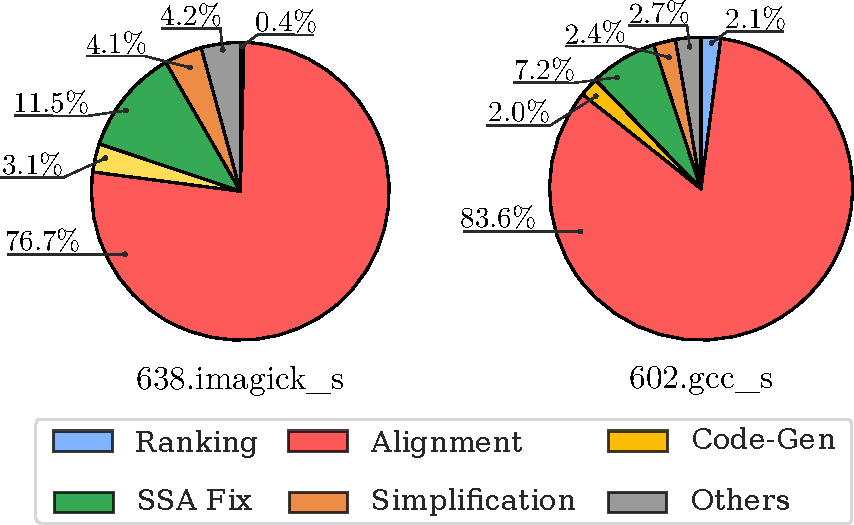
\includegraphics[width=0.7\linewidth]{src/lctes21/figs/compilation-breakdown-motivation-alignment.pdf}
  \caption{Breakdown of the relative runtime for the different stages from {\SOAName}. Alignment takes 25 seconds and 4.2 minutes on \texttt{638.imagick\_s} and \texttt{602.gcc\_s}, respectively.}
  \label{fig:compilation-breakdown-motivation-alignment}
\end{figure}

Most of the rest of the running time of function merging is associated with producing merged functions from the aligned sequences.
%\fixme{PP: Same suggestion as earlier about CodeGen.}
This includes the time spent on the code generation stage (Code-Gen), SSA reconstruction (SSA Fix), and code simplification (Simplification). These stages account for 18.7\% of the {\SOAName}’s running time on \texttt{638.imagick\_s} and 11.6\% on \texttt{602.gcc\_s}.
However, for other programs, these stages may represent the vast majority of {\SOAName}’s running time (see Section~\ref{sec:eval:pass-speedup}).

This breakdown includes the cost for producing both \emph{profitable} and \emph{unprofitable} merged functions.
In fact, most of it is wasted on merged functions that will be rejected by the profitability analysis.
These costs are pronounced because unprofitably merged functions have no limit on their size or complexity, often adding a significant pressure on the SSA reconstruction and simplification stages.
This effect is tied to the alignment strategy, since a good alignment is needed for producing profitably merged functions.
As we discuss in Section~\ref{sec:motivation:less-more}, a better approach would include a finer grain profitability analysis that would allows us to bail out from merging complex and unprofitable code as early as possible.

\subsection{When Less is More} \label{sec:motivation:less-more}

We observe that most of the benefit of function merging often comes from merging highly similar, but not necessarily identical, basic blocks. Figure~\ref{fig:xalan-example} shows one such example extracted from the \texttt{483.xalancbmk} benchmark found in SPEC CPU2006.
This example shows the two input functions annotated with the alignment produced by \SOAName. Merging these two functions contributes to a reduction of 33 bytes in the final object file.

\begin{figure}[h]
  \centering
  \includegraphics[width=\linewidth]{src/lctes21/figs/xalan-example.pdf}
  \caption{Example extracted from \texttt{483.xalancbmk} in SPEC CPU2006. Instructions marked green have been aligned through sequence alignment with an instruction from the other function. {\SOAName} would attempt merging all matched instructions but only the ones in fully aligned basic blocks would be profitable.}
  \label{fig:xalan-example}
\end{figure}

% \begin{figure*}[h]
%   \centering
%   \includegraphics[width=0.6\textwidth]{figs/xalan-example.pdf}
%   \caption{Example extracted from \texttt{483.xalancbmk} found in SPEC CPU2006.}
%   \label{fig:xalan-example}
% \end{figure*}

%This example also suggests that 
While this approach is flexible enough to identify very complex alignments, what it actually produces is three aligned pairs of basic blocks and a few aligned instructions in the entry blocks. More importantly, these entry block instructions offer nothing in terms of code size reduction. The gains of merging them are negated by the extra branches and operand selections needed to preserve the program's semantics. Since {\SOAName} analyzes the profitability of the final merged function as a whole, this unprofitable sequence of instructions will be merged because of the three highly profitable basic blocks. For the same reason, we may have profitable areas of code rejected because the rest of the merged function is unprofitable.


%Since {\SOAName} analyzes the profitability of the final merged function as a whole, we may have segments of unprofitably merged code inside an otherwise profitably merged function.
%Similarly, we may also have segments of profitably merged code inside merged functions that are thrown away by the profitability analysis. 
%However, we can achieve the same code size reduction of 33 bytes by merging only the subset of nearly identical basic blocks (highlighted in Figure~\ref{fig:xalan-example}).
%The gains of merging the entry blocks are negated by the extra branches and operand selections needed to preserve the program's semantics.

This example shows us that we could achieve similar code size reduction by breaking the problem of aligning functions into two simpler processes: first identifying highly similar basic blocks and then aligning the instructions in each pair of similar blocks. 
%merging functions on the basic block rather than on the instruction level adopted by \SOAName.
By operating on basic blocks, we could greatly reduce the length of the sequences to be aligned and the associated compilation and memory overhead. Furthermore, by making profitability decisions for each pair of basic blocks separately, we could avoid merging unprofitable pairs. The rest of this chapter shows how we use such an approach to overcome the weaknesses of \SOAName and make function merging practical for optimizing large programs. 

%Therefore, the main takeaways are:
%1) It often suffices to merge functions on a per basic block manner. %, since crossing the basic block boundary is rarely necessary.
%2) A fine-grain profitability analysis is needed to avoid  merging unprofitable pairs of basic blocks.



%This happens because the optimal sequence alignment algorithm used by SalSSA is trying to maximize the number of matching entries, which does not necessarily translate to the optimal merged function.
%Moreover, SalSSA is also limited by the fixed linearization strategy.
%For example, the two \textit{return} instructions are not aligned due to the ordering of the basic blocks chosen by the linearization strategy.

%We can take advantage of this insight in order to design a faster function merging technique.
%Ultimately, our goal is to be able to avoid the quadratic algorithm while still producing significant reductions to the program's size.

%In this paper, we take advantage of these key insights to propose a novel function merging technique that addresses the major overheads discussed in Section~\ref{sec:motivation:breakdown}.
%We can take advantage of this insight in order to design a better and faster function merging technique.
%To this end, we propose a novel function merging technique that work on the level of basic blocks and includes a fine-grain profitability analysis.



%bail out early from   of a fine-grain and a coarse-grain analysis.

%TODO: [Relatedwork] Note that this is different from the work done by von Koch~et~al.~\cite{edler14}, as these two functions are not \textit{structurally similar} as expected by their function merging technique and therefore could not be merged.


\input{src/cgo19/proposed}
\section{Evaluation}
\label{sec:evaluation}

In this section, we compare {\ProjName} against {\SOAName}, presented in Chapter~\ref{chp:pldi20}.
First, we evaluate the code size reduction achieved by each technique, demonstrating that our approach is on a par with {\SOAName}. Then we show that {\ProjName} reduces significantly the overhead of function merging. % to such a degree that it becomes negligible.
Combined with the speedup in later stages of the compilation pipeline due to the reduced amount of code, {\ProjName} leads to faster end-to-end compilation than a baseline with no function merging enabled. Finally, we demonstrate how our contributions reduce the memory usage by several orders of magnitude. 

\subsection{Experimental Setup}
%We compare {\ProjName}, our novel function merging technique, against {\SOAName}, the  state-of-the-art~\cite{rocha20}.
In addition to evaluating \SOAName, we also consider four variations of our technique based on two dimensions:
1) the linear Pairwise Alignment (PA) versus the quadratic {\NW} Alignment (NW), both on a per basic block manner and
2) using a multi-tier profitability analysis versus using only the standard profitability analysis from {\SOAName}, which is the analysis applied on the whole function after generating the merged function.
As described in Section~\ref{sec:contribution}, the [PA] variant is, by construction, limited to merging only basic blocks of the same size. The [NW] variant can merge blocks of different sizes. The four variations are:

\begin{itemize}
    \item {[PA]}: PA with the Multi-tier Profitability analysis.
    \item {[PA,NMP]}: PA with No Multi-tier Profitability.
    \item {[NW]}: NW with the Multi-tier Profitability.
    \item {[NW,NMP]}: NW with No Multi-tier Profitability.
    %\item {[NW,SS]}: NW with Block Profitability but applied on blocks of the Same Size (SS).
\end{itemize}

%For \SOAName, we used the version published in their evaluation artifact~\cite{SalSSA}.
To keep the comparison fair, we implemented {\ProjName} for the same compiler as \SOAName, LLVM \fixme{v11}. We evaluated all techniques on the C/C++ programs from the SPEC CPU 2006 and the SPEC CPU 2017 benchmark suites~\cite{spec}. The baseline in all cases is the LLVM build in full LTO mode without any function merging.

We target the Intel x86 architecture.
All experiments were performed on a dedicated server with a quad-core Intel Xeon CPU E5-2650, 64 GiB of RAM, running Ubuntu 18.04.3 LTS. To minimize the effect of measurement noise, we repeated all compilation and runtime overhead experiments 5 times. We report the average values and their 95\% confidence intervals.

We evaluate all approaches in terms of code size reduction, time overhead of function merging, end-to-end compilation time, and peak memory usage. To better examine the trade-off between code size reduction and compilation time, we also introduce and measure a new metric called \textit{average reduction speed} which shows the efficiency of the optimization at reducing code size. This metric offers a single number that allows us to compare how different versions address the trade-off between compilation time and code size reduction.

\begin{definition}[Average Reduction Speed]
For a given input program and optimization, let $S$ and $S_0$ be the size of the program with and without the given optimization, respectively.
$R = S_0 - S$ represents the reduction achieved by such optimization.
Let $T$ be the running time of the optimization pass.
We define the \textit{average reduction speed} as:
\[
   ARS = \frac{R}{T}
\]  
\end{definition}

\subsection{Code Size Reduction} \label{sec:eval:size}

Figures~\ref{fig:size-reduction-both} reports the reduction on the size of the linked object files produced by the compiler.
While limiting alignment at a basic block granularity seems restrictive, its effect on code size is small. Even the worst performing variants of {\ProjName} are still within 3 percentage points of {\SOAName}, while both [PA] and [NW] achieve good results that are on a par with {\SOAName}. [PA]'s code size reduction varies from 5 percentage points worse to over 10 points better than {\SOAName}. On average, it is within 1 percentage point of the reduction achieved by {\SOAName}. [NW] almost always achieves better code size reduction than [PA] and on average outperforms {\SOAName} by a small margin. Since our primary aim is to reduce the high compile-time overheads of {\SOAName}
%, in the following sections,
a small loss of code reduction is acceptable. 

 \begin{figure}[h]
   \centering
 \begin{subfigure}{\textwidth}
 \center
   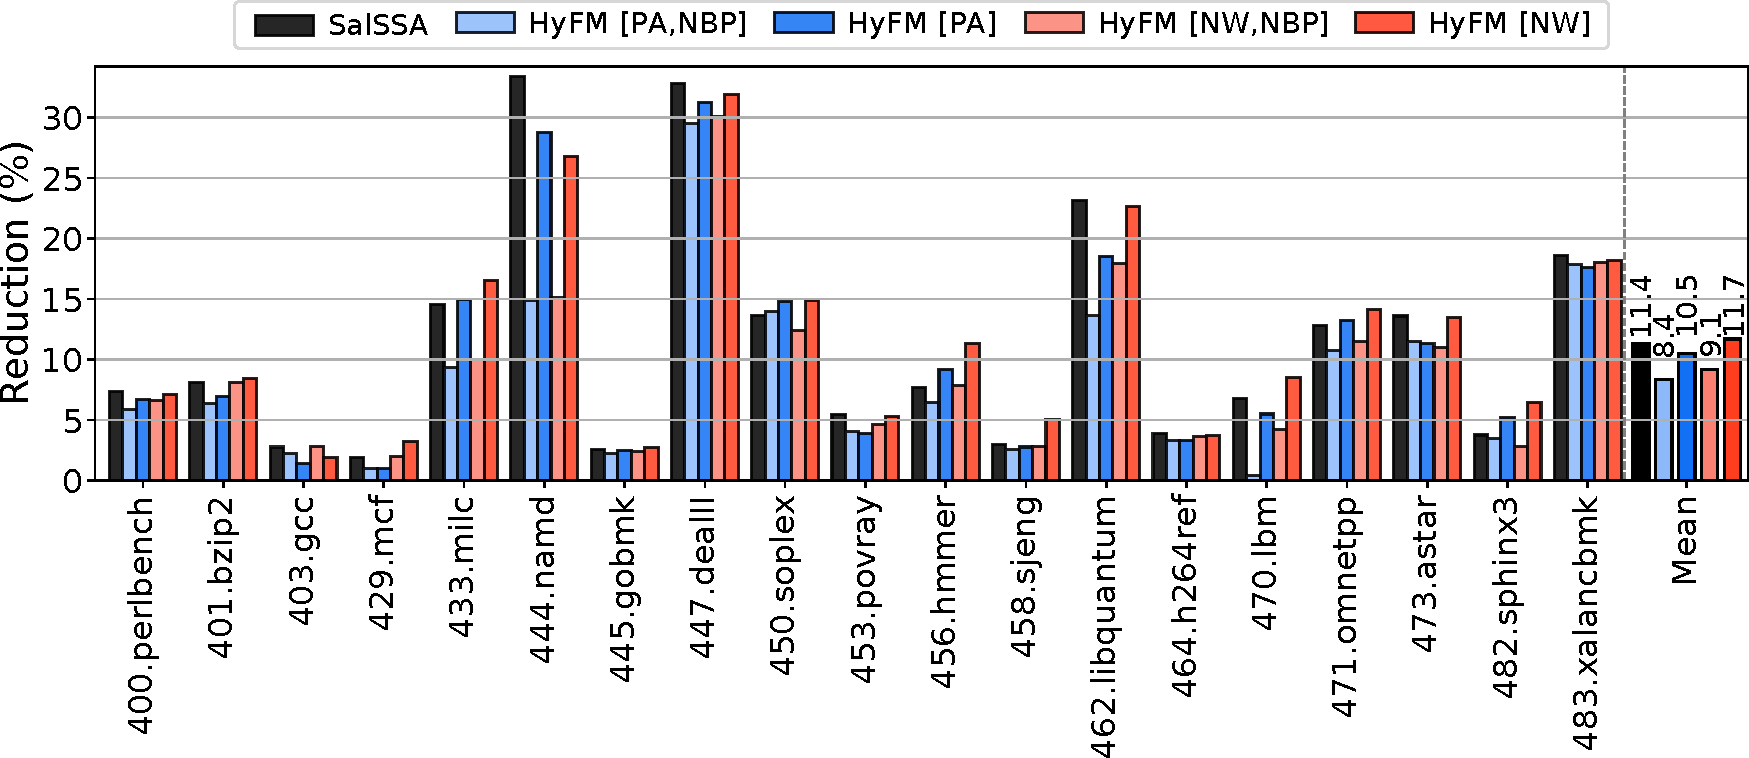
\includegraphics[width=\textwidth]{src/lctes21/figs/reduction-spec06.pdf}
 \caption{SPEC CPU 2006.}
 \label{fig:size-reduction-spec06}
 \end{subfigure}
 \\
 \begin{subfigure}{\textwidth}
 \center
   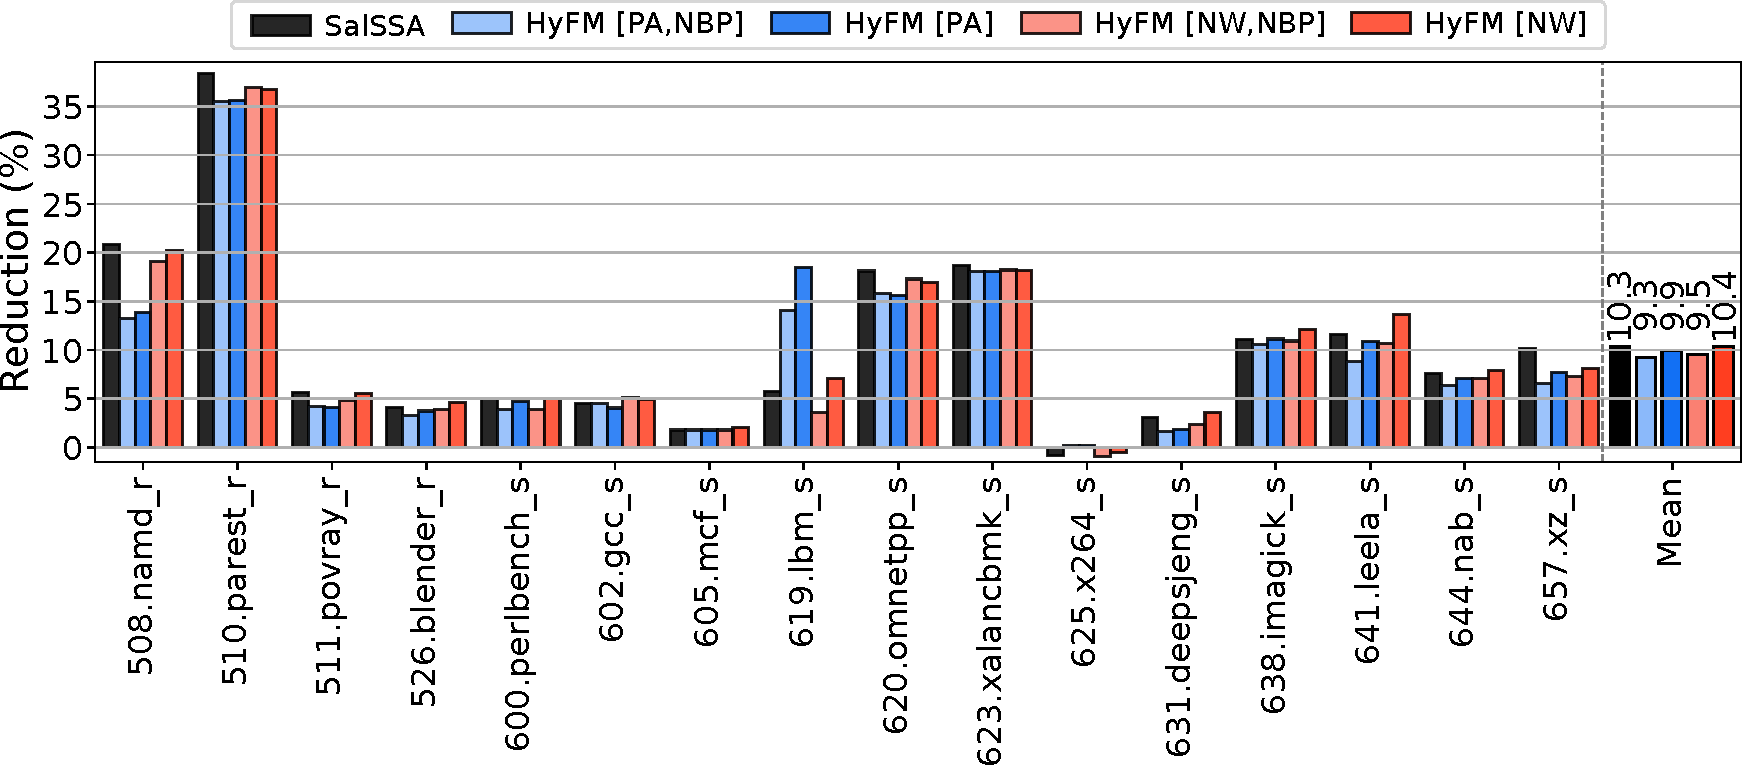
\includegraphics[width=\textwidth]{src/lctes21/figs/reduction-spec17.pdf}
 \caption{SPEC CPU 2017.}
 \label{fig:size-reduction-spec17}
 \end{subfigure}
 \caption{Linked object size reduction over LLVM LTO
      when performing function merging with {\ProjName} or {\SOAName} on SPEC CPU 2006 and 2017. On average, {\ProjName} improves code size reduction.}
  \label{fig:size-reduction-both}
 \end{figure}

%\begin{figure*}[t]
%  \centering
%  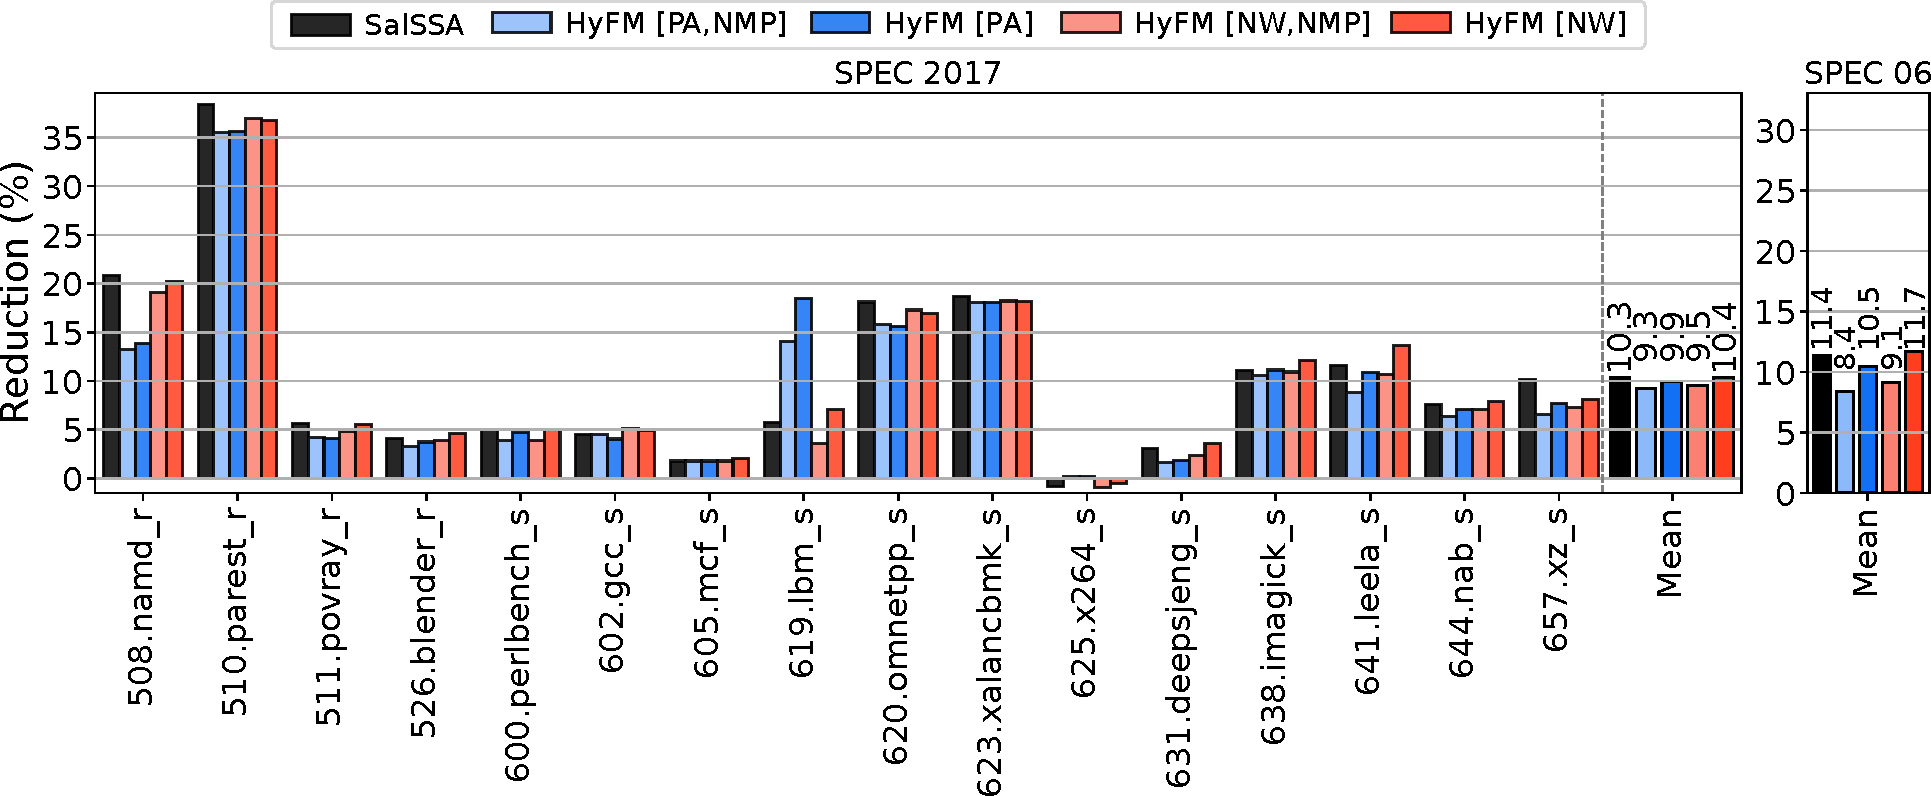
\includegraphics[width=0.95\linewidth]{src/lctes21/figs/reduction-spec17-06.pdf}
%  \caption{Linked object size reduction over LLVM LTO
%      when performing function merging with {\ProjName} or {\SOAName} on SPEC CPU 2006 and 2017. On average, {\ProjName} improves code size reduction.}
%  \label{fig:size-reduction-both}
%\end{figure*}

%Overall, {\ProjName} is on a par with the state of the art {\SOAName}.
%Since our primary aim is to reduce the high compile-time overheads of function merging, as described in Sections~\ref{sec:eval:compilation-time} and \ref{sec:eval:memory}, a small loss of code size reduction is acceptable.

%Even though restricting merging exclusively to basic blocks of the same size seems, at first glance, excessively strong, its effect on code size reduction is limited. On average, same size blocks lead to less than 1\% change compared to the state of the art.

These results indicate that the multi-tier profitability analysis is the single most important component of our approach. 
The two variants without the multi-tier profitability analysis, [PA,NMP] and [NW,NMP], are consistently worse than their counterparts that include this analysis, i.e. [PA] and [NW]. The multi-tier analysis contributes on average about 1 percentage point in code reduction for SPEC 2017 and more than 2 points for SPEC 2006.
The multi-tier profitability analysis has an important impact in the quality of the merged function.
While {\SOAName} lets unprofitable merged subsequences through as long as they are outweighed by profitable subsequences elsewhere in the merged function, {\ProjName} filters such unprofitable subsequences out.

The next most important effect comes from the choice of alignment algorithm. {\NW} is on average half a percentage point better than Pairwise Alignment for SPEC 2017 and about one percentage point better for SPEC 2006. Given that Pairwise Alignment only aligns blocks of the same size and does not try to discover optimal alignments, this difference is smaller than one would expect.
It indicates that profitable pairs of basic blocks tend to be extremely similar if not identical, as discussed in Section~\ref{sec:motivation}.
Still, {\NW} results in more size reduction.
When code size reduction is paramount, [NW] might be a better choice than [PA], but as we will see in Sections~\ref{sec:eval:compilation-time} and \ref{sec:eval:memory}, there is still a trade-off to navigate.

We get the biggest improvement by {[PA]} compared to {\SOAName} and {[NW]} for \texttt{lbm}, where it reduces the program's object file by 18.5\%, almost 13 percentage points more than the competition.
%%%%%%It's actually merging a few profitable basic blocks while giving up on several unprofitable merge sequences
%This comes from discovering a merging opportunity between two large basic blocks of the same size.
%Both {[PA]} and {[PA,NMP]} try merging these blocks but {\SOAName}, {[NW]}, and {[NW,NMP]} choose to focus on other candidates. Compared to {[PA,NMP]}, {[PA]} also finds and profitably merges the same function as {\SOAName} leading to even higher code size reduction.
{\SOAName} is able to profitably merge two pairs of functions.
On the other hand, {[PA,NMP]} chooses to perform a chained merge of the three largest functions in \texttt{lbm}, resulting in a significantly smaller binary.
This is possible because {[PA,NMP]} is merging some nearly identical pairs of basic blocks of the same size.
With the multi-tier profitability analysis, {[PA]} successfully identifies all four cases. 
{[NW]} fails to identify all of these cases, even though it is still better than {\SOAName}.
This exposes existing limitations in the cost model used by our profitability analysis.
%\fixme{Is this a cost model problem?}

The two worst results for {[PA]} are for the \texttt{namd} benchmark in both SPEC 2006 and SPEC 2017. {\SOAName} achieves close to 7 percentage points more than {[PA]} in code size reduction.
In both cases, Pairwise Alignment limits the number of successful merge operations. The variants using {\NW} recover most of the lost reduction. 

% \begin{figure}[h]
%   \centering
%   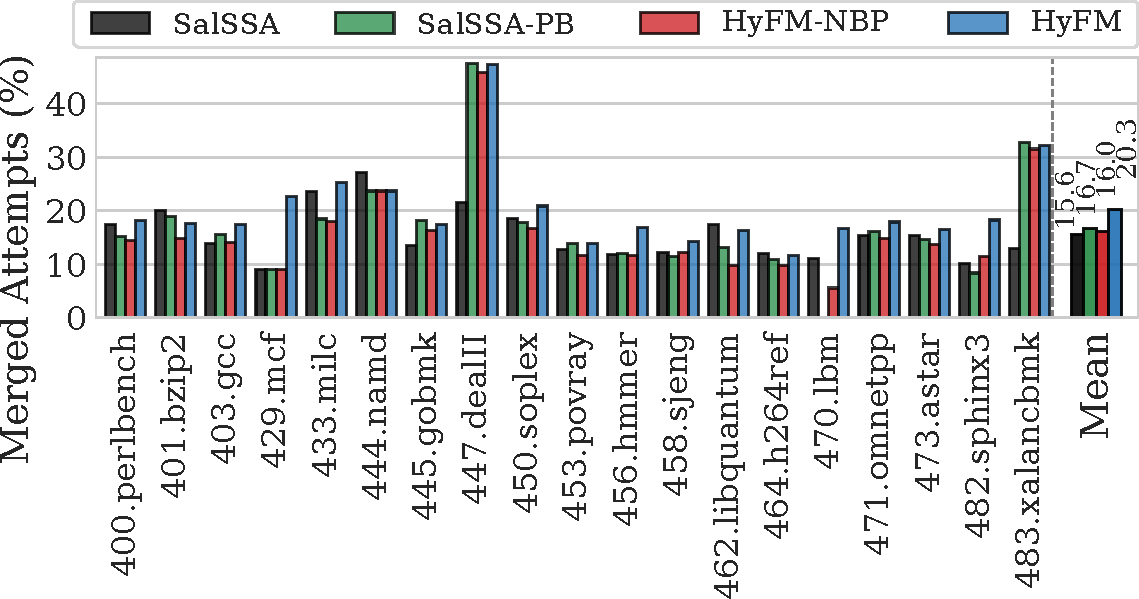
\includegraphics[width=\linewidth]{figs/merged-attempts-perc-spec06.pdf}
%   \caption{Number successful merging attempts on SPEC 2006.}
%   \label{fig:merged-attempts-perc-spec06}
% \end{figure}

% \begin{figure}[h]
%   \centering
%   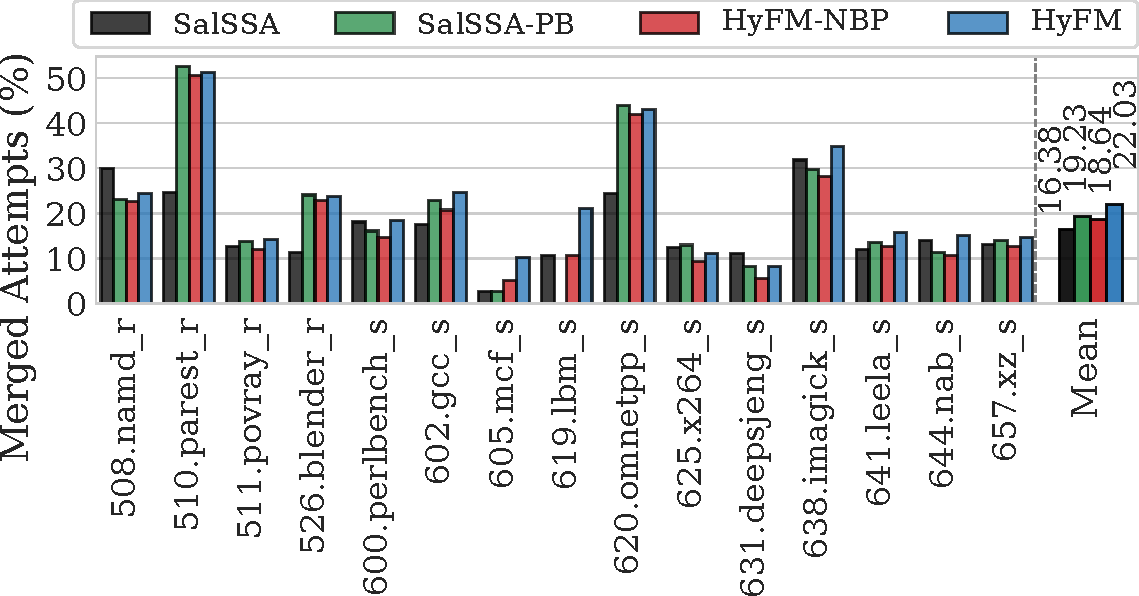
\includegraphics[width=\linewidth]{figs/merged-attempts-perc-spec17.pdf}
%   \caption{Number of successful merging attempts on SPEC 2017.}
%   \label{fig:merged-attempts-perc-spec17}
% \end{figure}

% \begin{figure}[h]
%   \centering
%   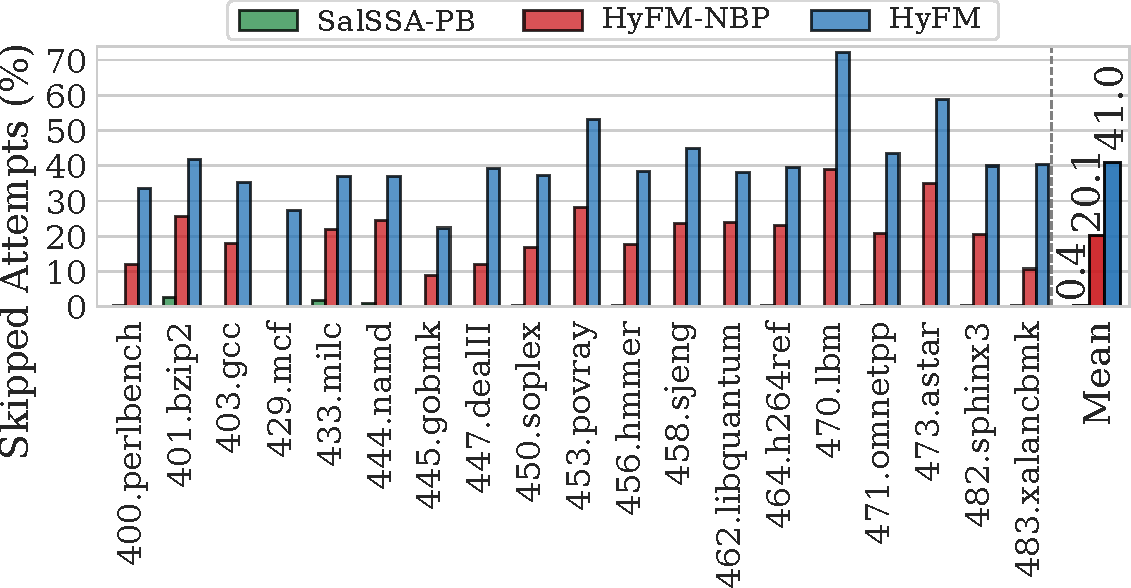
\includegraphics[width=\linewidth]{figs/skipped-attempts-perc-spec06.pdf}
%   \caption{Number of skipped merging attempts on SPEC 2006.}
%   \label{fig:skipped-attempts-perc-spec06}
% \end{figure}

% \begin{figure}[h]
%   \centering
%   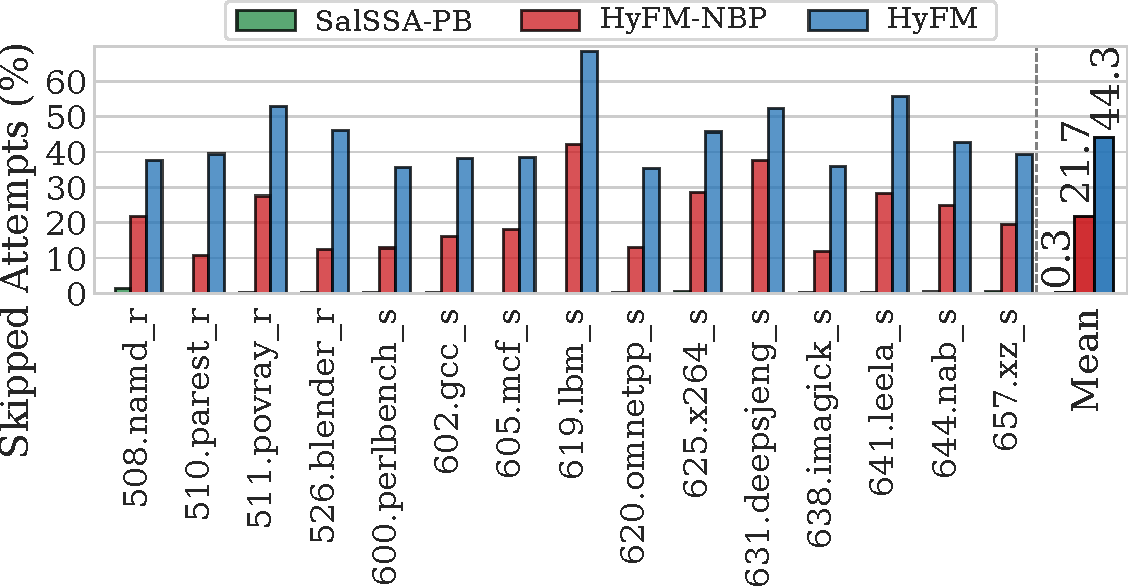
\includegraphics[width=\linewidth]{figs/skipped-attempts-perc-spec17.pdf}
%   \caption{Number of skipped merging attempts on SPEC 2017.}
%   \label{fig:skipped-attempts-perc-spec17}
% \end{figure}


% \begin{figure*}[h]
%   \centering
%   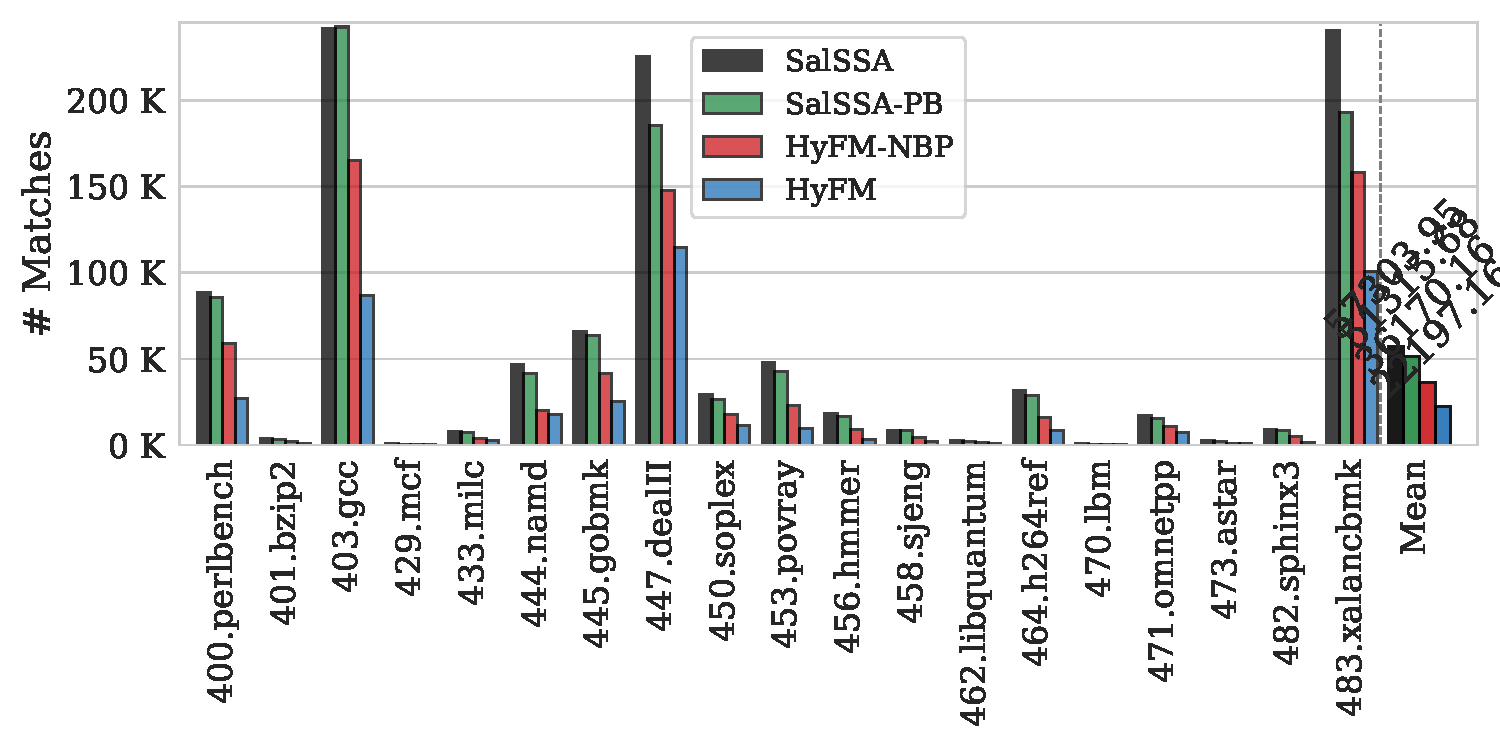
\includegraphics[width=0.85\linewidth]{figs/total-num-matches-spec06.pdf}
%   \caption{Total number of matching entries, including profitable and unprofitable attempts. SPEC 2006.}
%   \label{fig:total-num-matches-spec06}
% \end{figure*}

% \begin{figure*}[h]
%   \centering
%   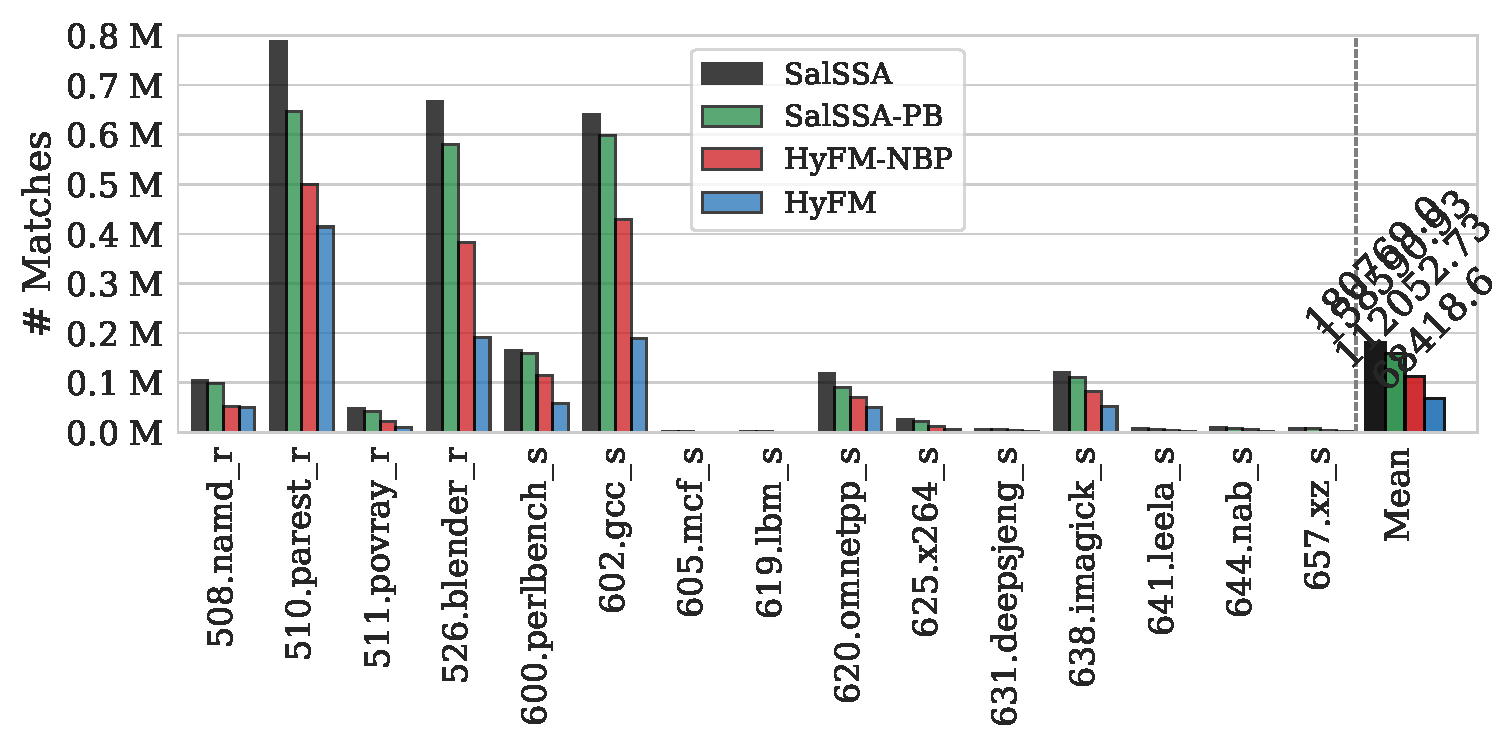
\includegraphics[width=0.85\linewidth]{figs/total-num-matches-spec17.pdf}
%   \caption{Total number of matching entries, including profitable and unprofitable attempts. SPEC 2017.}
%   \label{fig:total-num-matches-spec17}
% \end{figure*}

\subsection{Speeding Up Function Merging} \label{sec:eval:pass-speedup}

 \begin{figure}[h]
   \centering
 \begin{subfigure}{\textwidth}
 \center
   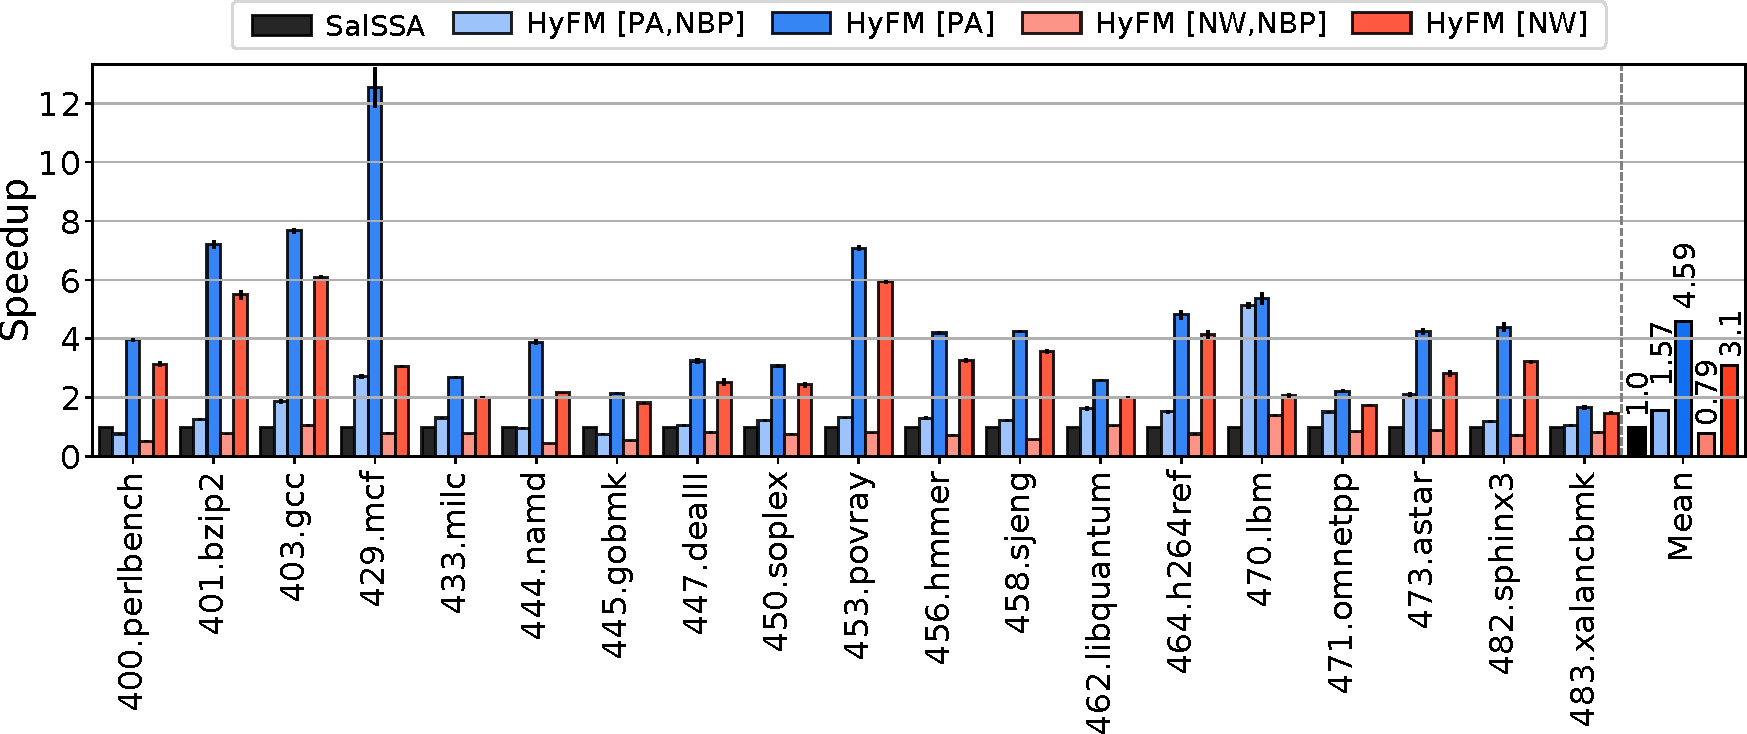
\includegraphics[width=\textwidth]{src/lctes21/figs/speedup-spec06.pdf}
 \caption{SPEC CPU 2006.}
 \label{fig:speedup-spec06}
 \end{subfigure}
 \\
 \begin{subfigure}{\textwidth}
 \center
   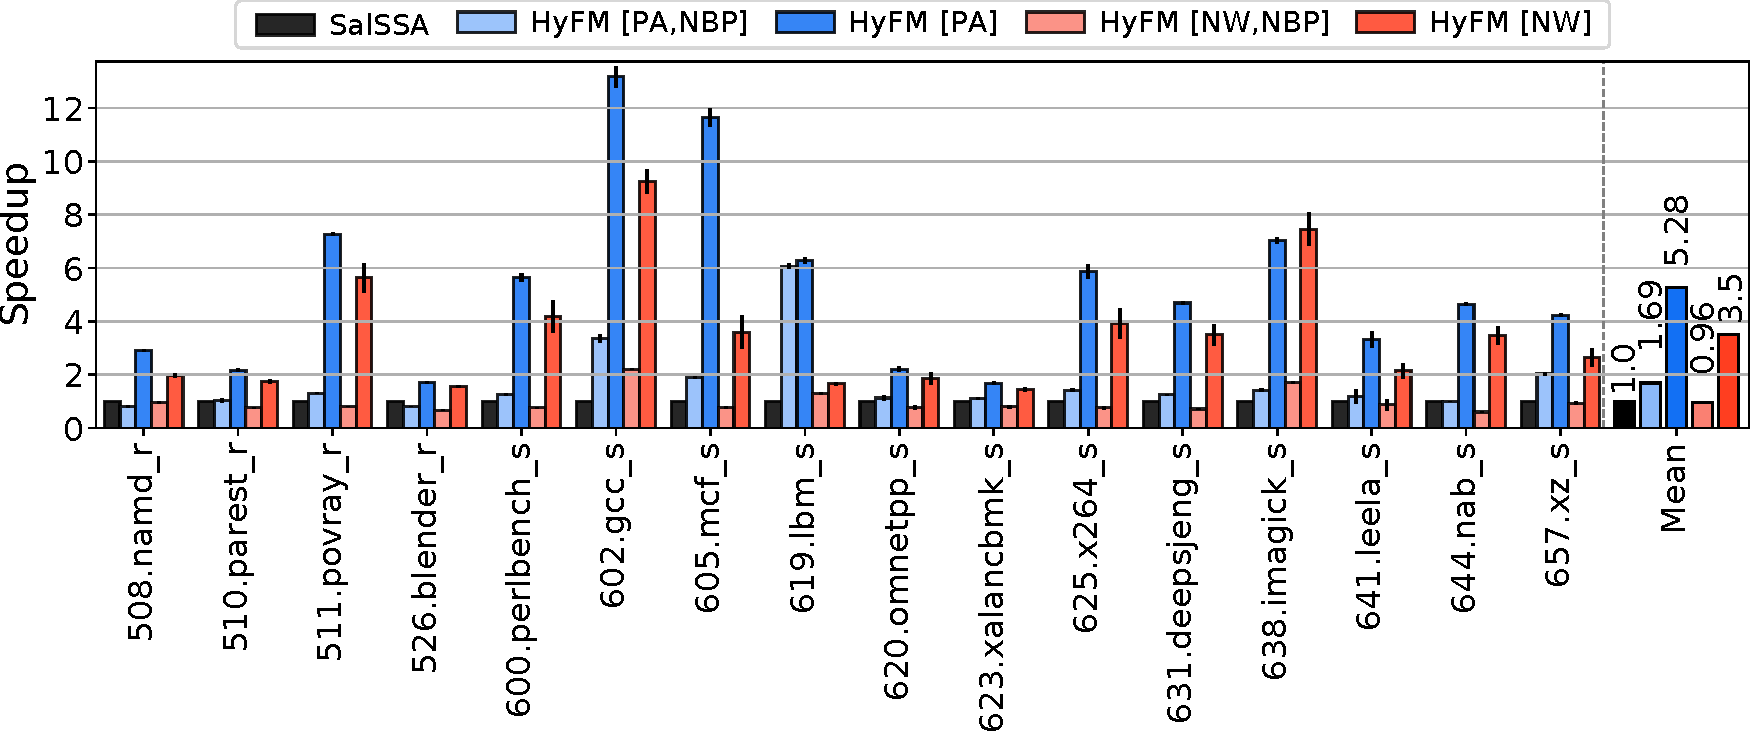
\includegraphics[width=\textwidth]{src/lctes21/figs/speedup-spec17.pdf}
 \caption{SPEC CPU 2017.}
 \label{fig:speedup-spec17}
 \end{subfigure}
 \caption{Speedup of the function merging pass in isolation relative to {\SOAName}. The multi-tier profitability analysis reduces the number of unprofitable merge operations leading to a significant speedup.}
  \label{fig:speedup-both}
 \end{figure}

%\begin{figure*}[t]
%  \centering
%  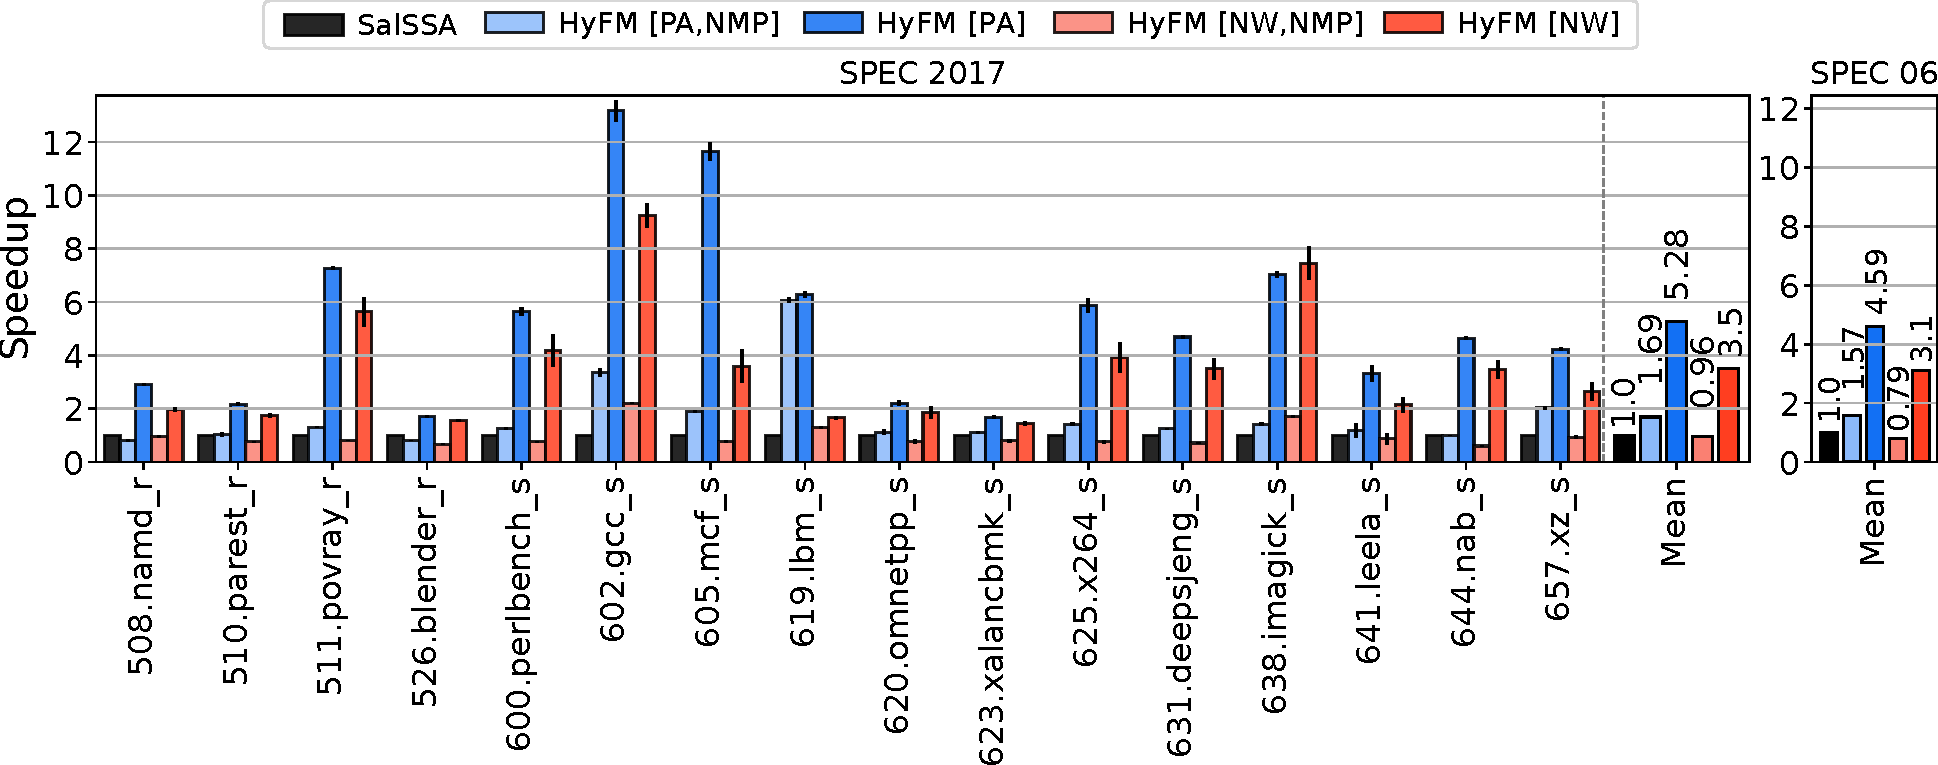
\includegraphics[width=0.95\linewidth]{src/lctes21/figs/speedup-spec17-06.pdf}
%  \caption{Speedup of the function merging pass in isolation relative to {\SOAName}. The multi-tier profitability analysis reduces the number of unprofitable merge operations leading to a significant speedup.}
%  \label{fig:speedup-both}
%\end{figure*}

Figure~\ref{fig:speedup-both} shows the speedup of {\ProjName} relative to {\SOAName}.
This considers only the time taken by the function merging pass, which include all stages discussed in Section~\ref{sec:motivation:breakdown}.
Our novel technique achieves an impressive speedup. For {[PA]} it is on average $5.28\times$ faster for SPEC 2017 and $4.59\times$ for SPEC 2006. Even in the worst case, it achieves a \fixme{50}\% speedup. In the best case, for the SPEC 2017 \texttt{gcc}, function merging under {\ProjName} takes a total of 23.5 seconds instead of 302, which translates to almost $13\times$ less time.

%The two variants with the multi-tier profitability analysis achieve on average three to four times higher speedups than their counterparts without it. This is a direct result of bailing out early. For most benchmarks, only a small number of candidate pairs is profitable. The majority are unprofitable but SalSSA has to merge them anyway to determine their profitability. This is expensive and wasteful. Our approach,on the other hand, is able to estimate profitability early. Only function pairs with any chance of being profitable, that is pairs with at least one profitable pair of basic blocks, move forward to the expensive merge stage.
%The linear pairwise alignment contributes to the performance improvement, too. The variants using pairwise alignment run on average 48% to 98% faster than their Needleman-Wunsch counterparts. The most pronounced case is for lbm where [PA] is around3×faster than [NW]. The blocks paired in lbm are longer than usual, so the quadratic Needleman-Wunsch spends significantly more time trying to align them than our linear pairwise algorithm. Figure 7 shows that the added pairing restrictions from [PA], to focus on blocks with higher similarities, also benefits later stages.
%All components of HyFM contribute towards this result but the multi-tier profitability analysis has the most significant impact. As we show in Figure 7, even though the time spent on the alignment strategy becomes negligible for both [PA,NMP] and [PA], the lack of a multi-tier profitability analysis may degrade the stages associated with code generation. If we accept the alignment for any pair of basic blocks, we may end up producing complex merged functions— code with an excessive amount of branches, phi-nodes,and operand selections — slowing down SSA reconstruction and code simplification. This effect can be observed with [PA,NMP] for many benchmarks in Figure 7. Most notably, for the blender benchmark, [PA,NMP] is slower than SalSSA due to its added pressure on the SSA reconstruction algorithm, even though its alignment strategy runs much faster. For this reason, enabling the multi-tier profitability analysis has a positive impact on later stages.

All components of {\ProjName} contribute towards this result but the multi-tier profitability analysis has the most significant impact. The two variants with the multi-tier profitability analysis achieve on average three to four times higher speedups than their counterparts without it.
To help us understand why, Figure~\ref{fig:breakdown-spec17} shows how the compilation time of each approach is distributed across its various stages. 
Even though the time spent on the alignment strategy becomes negligible with {\ProjName}, the less optimal alignment often produces complex merged functions --- code with an excessive amount of branches, phi-nodes, and operand selections --- slowing down SSA reconstruction and code simplification. This effect is very pronounced for the \texttt{blender} benchmark, where both [PA,NMP] and [NW,NMP] are slower than {\SOAName} due to the added pressure on the SSA reconstruction algorithm, even though the alignment overhead is practically zero.
Similar effects can be observed in other benchmarks.

\begin{figure}[h]
  \centering
  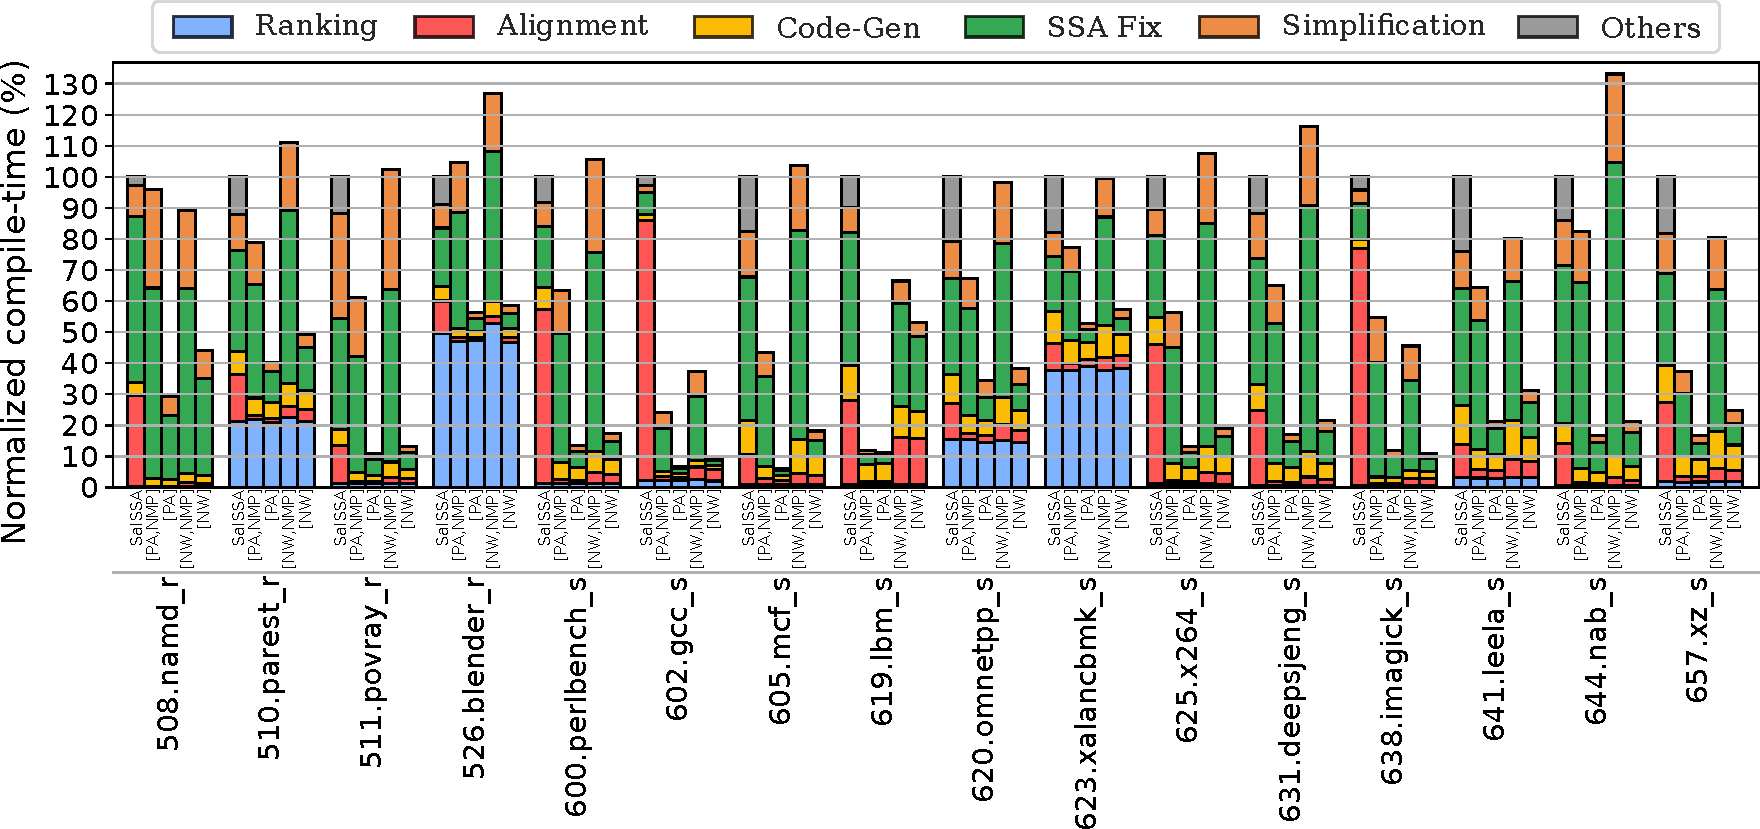
\includegraphics[width=\linewidth]{src/lctes21/figs/breakdown-full-spec17.pdf}
  \caption{Breakdown of the relative runtime for the different stages of the function merging pass. All measurements are normlized by \SOAName's total runtime on the corresponding benchmark. For every benchmark, we show {\SOAName}, [PA,NMP], [PA], [NW,NMP], and [NW], in this order. }
  \label{fig:breakdown-spec17}
\end{figure}

Enabling the multi-tier profitability analysis counters this effect by focusing code generation exclusively on profitable blocks and functions. Most of the complex basic blocks {\ProjName} generates are not profitable for the same reason it is expensive to process them. First-tier profitability filters them out. On top of that, most paired functions under either {\SOAName} or {\ProjName} are unprofitable. {\SOAName} has to merge them anyway to determine their profitability. This is expensive and wasteful. Our approach, on the other hand, is able to estimate profitability early. Only function pairs with any chance of being profitable, that is pairs with at least one profitable pair of basic blocks, move forward to the expensive merge stage.

The linear pairwise alignment contributes to the performance improvement, too. The variants using pairwise alignment run on average 48\% to 98\% faster than their {\NW} counterparts.
%The most pronounced case is for \texttt{mcf} where {[PA]} is approximately $3\times$ faster than {[NW]}. Candidate basic block pairs in \texttt{mcf} are longer than usual, so the quadratic {\NW} spends significantly more time trying to align them than our linear pairwise algorithm. 
The most pronounced case is for \texttt{lbm} where {[PA]} is around $3\times$ faster than {[NW]}. The blocks paired in \texttt{lbm} are longer than usual, so the quadratic {\NW} spends significantly more time trying to align them than our linear pairwise algorithm.
Figure~\ref{fig:breakdown-spec17} shows that the added pairing restrictions from [PA], to focus on blocks with higher similarities, also benefits later stages.

\subsection{End-to-End Compilation Time} \label{sec:eval:compilation-time}

We have also analyzed separately the end-to-end compilation time because reducing code size through function merging has knock-on effects in later stages of the compilation pipeline.
The first order effect is that reducing the number of functions tends to reduce compilation time.
This is not guaranteed though, because merged functions may be more complex, potentially slowing down later compiler analyses and transformations.
Moreover, the time spent merging functions may be so large that it negates any benefits from having fewer functions later in the pipeline.

Even though on a few occasions {\SOAName} reduces end-to-end compilation time, in general, its overhead is large enough to result in an overall compilation time slowdown, 9.5\% to 4.1\% for SPEC 2017 and 2006 respectively.
In contrast, {\ProjName} is so much faster that its compilation time overhead is matched or outweighed by the speedup in later stages. 
This reduction is marginal for SPEC 2017, but for SPEC 2006 {[PA]} reduces the average compilation time by 2.3\% and {[NW]} by 1.6\%.
There is only a single case where {[PA]} results in a significant end-to-end slowdown, 10\% for \texttt{blender}.
%While this is still an improvement compared to {\SOAName}, \fixme{EXPLAIN}.
Figure~\ref{fig:breakdown-spec17} shows that, although [PA] runs faster than {\SOAName}, both of them spent a significant amount of time ranking the function candidates, due to its large number of functions.
Ranking alone in this case takes around 70 seconds. %However, this is beyond the scope of this paper.

Overall, we believe that this reduction in end-to-end compilation time is a very important result. While {\ProjName} is still achieving code-size reduction on par with the state-of-the-art, it does not have the detrimental effects of {\SOAName} on the overall compilation process and can be safely applied.

 \begin{figure}[h]
   \centering
 \begin{subfigure}{\textwidth}
 \center
   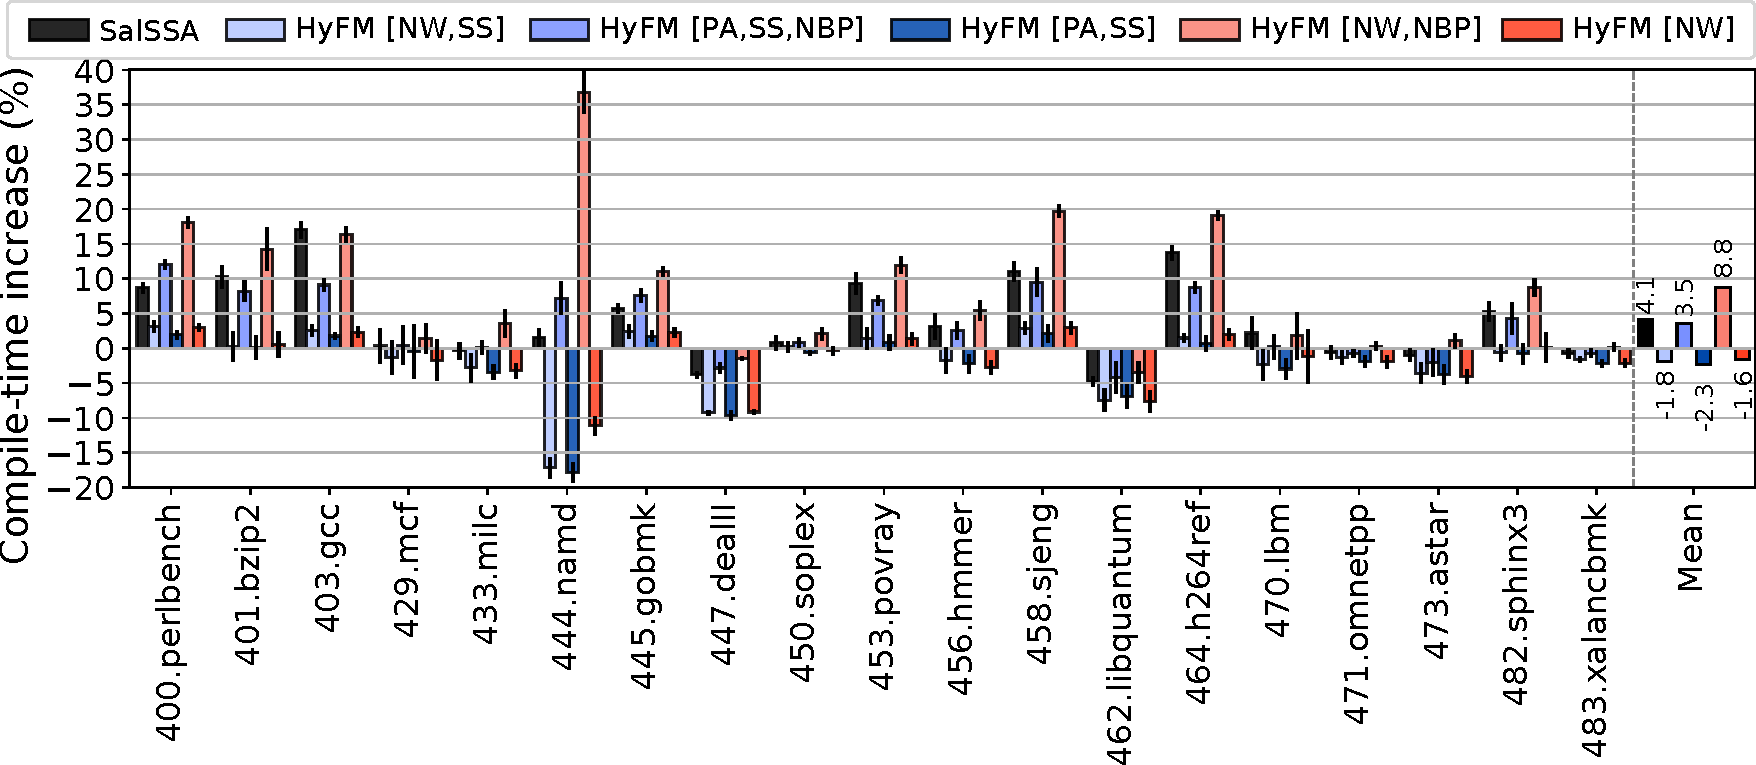
\includegraphics[width=\textwidth]{src/lctes21/figs/compiletime-spec06.pdf}
 \caption{SPEC CPU 2006.}
 \label{fig:compiletime-spec06}
 \end{subfigure}
 \\
 \begin{subfigure}{\textwidth}
 \center
   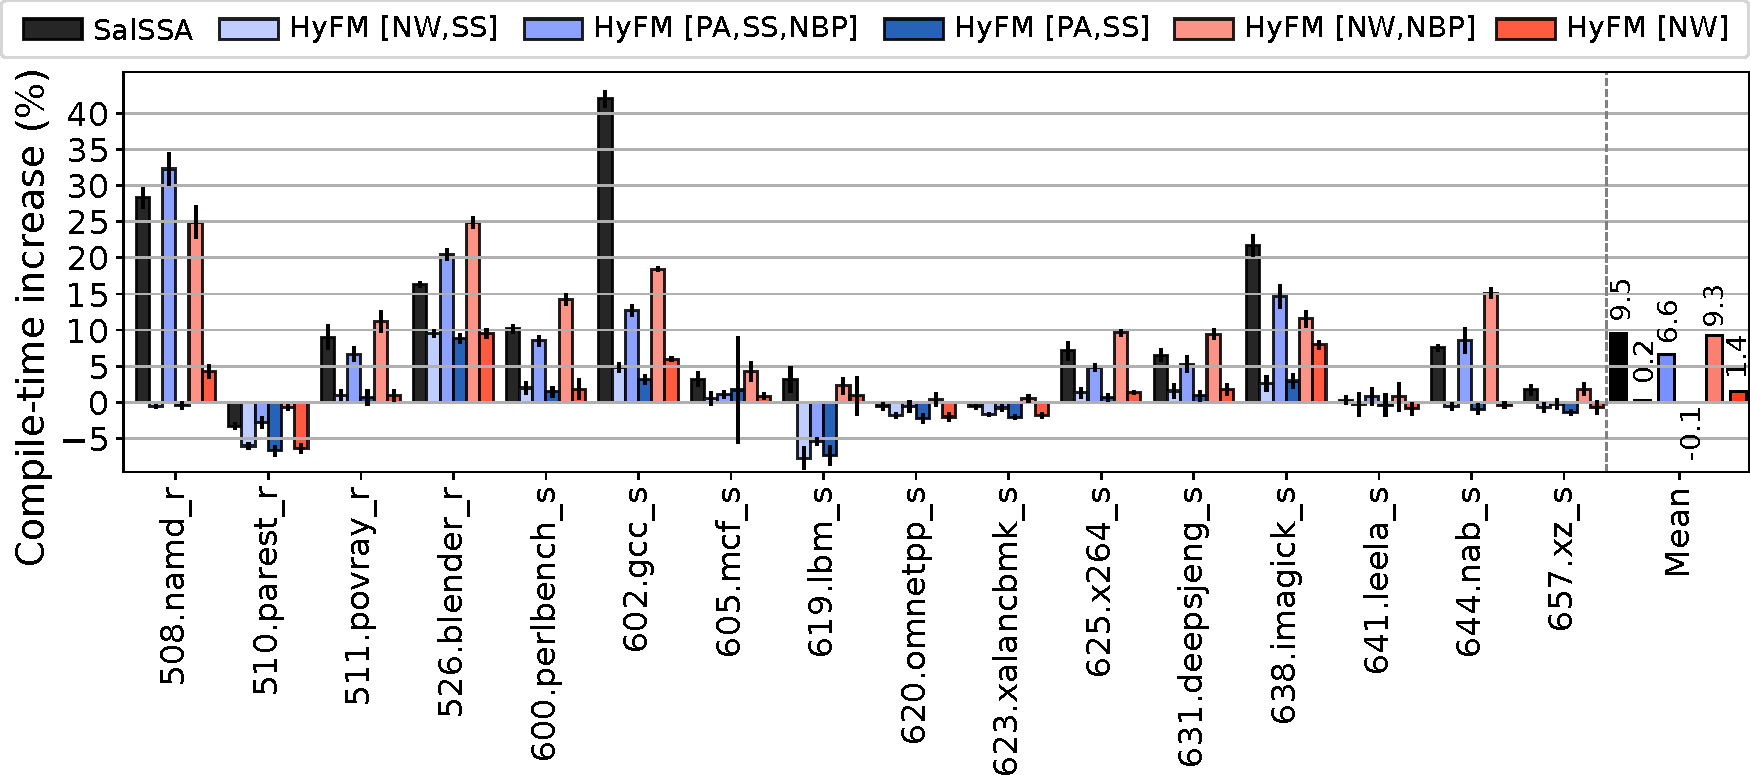
\includegraphics[width=\textwidth]{src/lctes21/figs/compiletime-spec17.pdf}
 \caption{SPEC CPU 2017.}
 \label{fig:compiletime-spec17}
 \end{subfigure}
 \caption{Normalized end-to-end compilation time for SPEC 2017 and SPEC 2006 relative to LLVM LTO.}
  \label{fig:compiletime-both}
 \end{figure}

%\begin{figure*}[h]
%  \centering
%  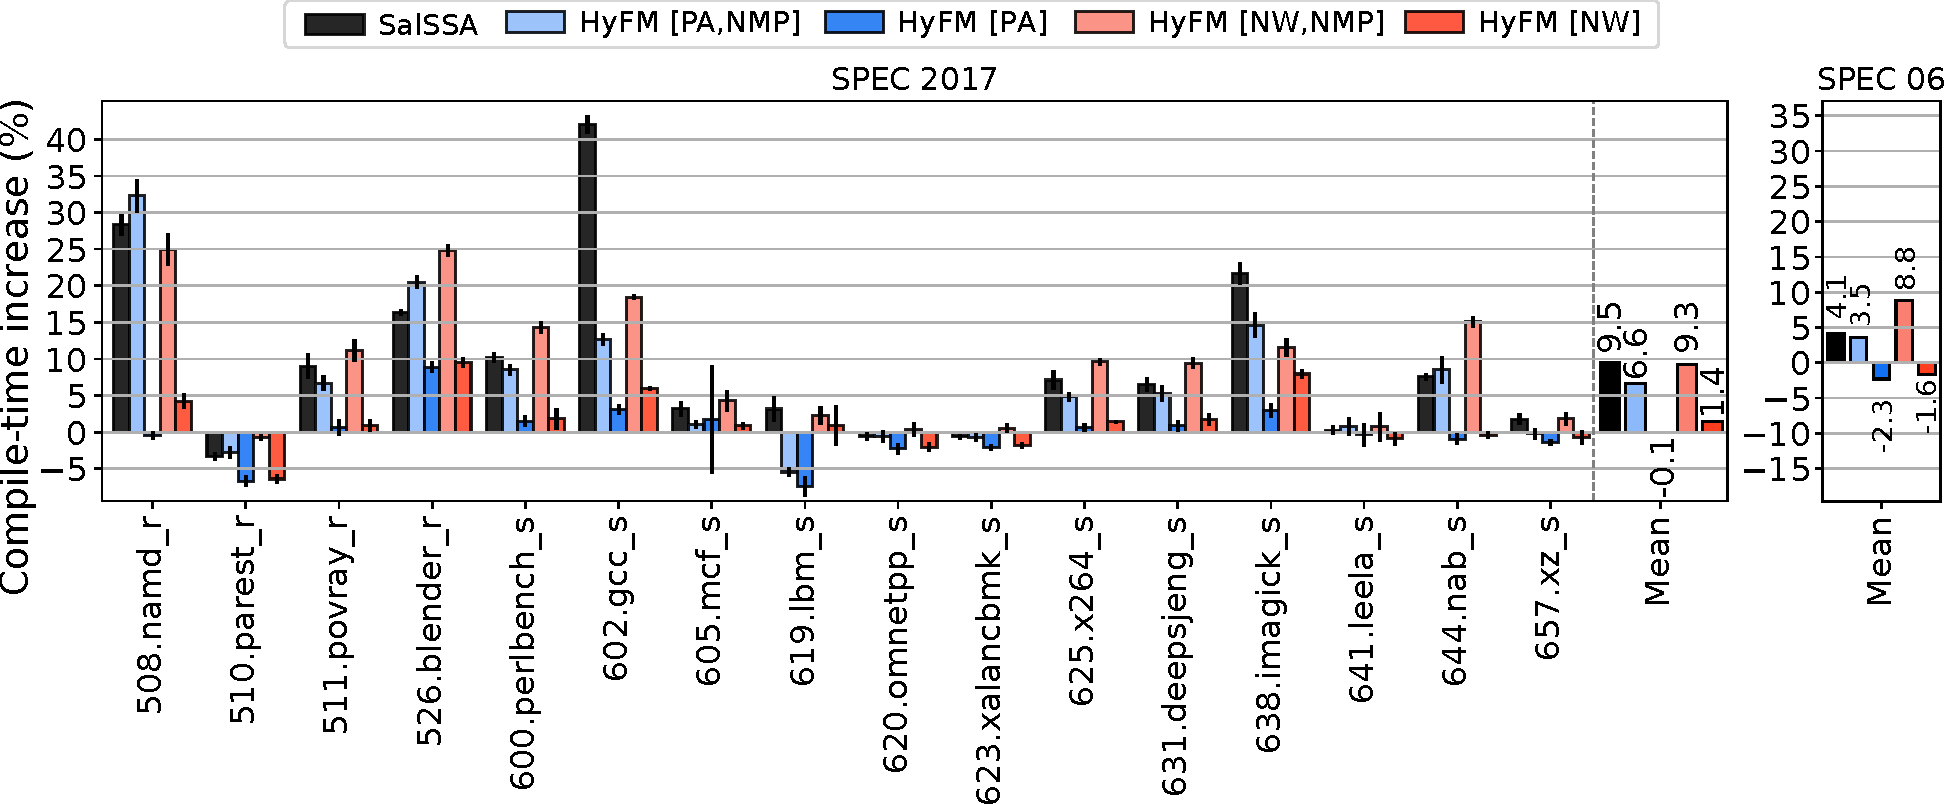
\includegraphics[width=0.95\linewidth]{src/lctes21/figs/compiletime-spec17-06.pdf}
%  \caption{Normalized end-to-end compilation time for SPEC 2017 and SPEC 2006 relative to LLVM LTO.}
%  \label{fig:compilation-both}
%\end{figure*}


\subsection{Code Size and Compilation Time Trade-Off} \label{sec:eval:trade-off}

While the multi-tier profitability analysis improves both code-size reduction and compilation speed, the choice of alignment algorithm introduces a trade-off. Pairwise alignment is better for speed, {\NW} is better for code-size reduction. 
In terms of compilation efficiency, i.e. how much code size reduction we get for the effort we put in, the picture is clearer. In Figure~\ref{fig:ars-both}, the \textit{average reduction speed} suggests that {[PA]} achieves the ideal trade-off, with an average reduction speed of 115.3~KB/s, which is around $3\times$ greater than {\SOAName}'s and 20\% to 40\% greater than [NW].


 \begin{figure}[h]
   \centering
 \begin{subfigure}{\textwidth}
 \center
   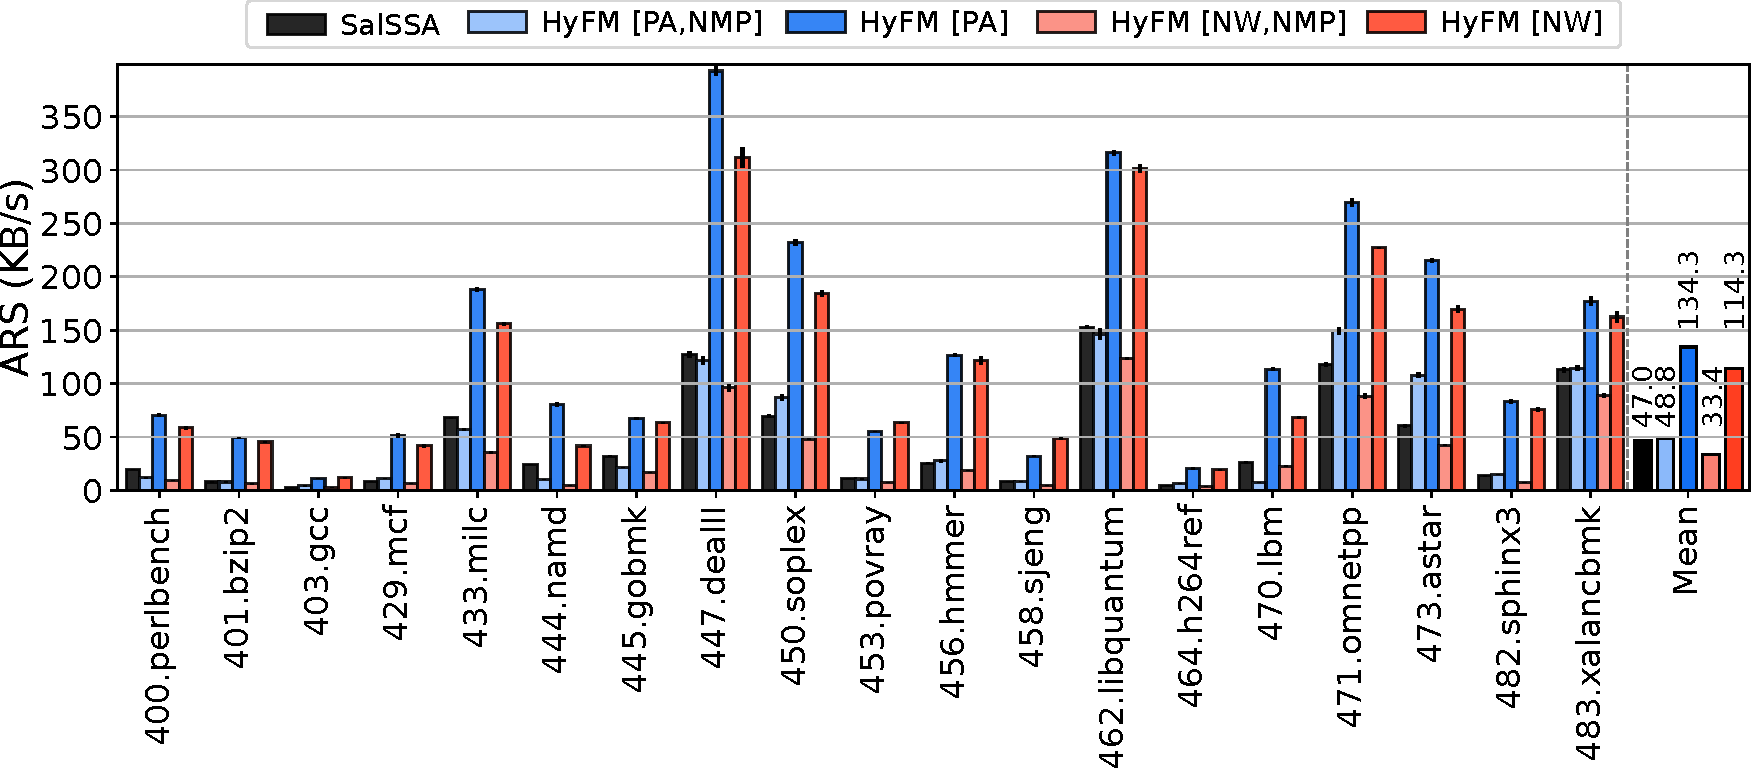
\includegraphics[width=\textwidth]{src/lctes21/figs/ars-spec06.pdf}
 \caption{SPEC CPU 2006.}
 \label{fig:ars-spec06}
 \end{subfigure}
 \\
 \begin{subfigure}{\textwidth}
 \center
   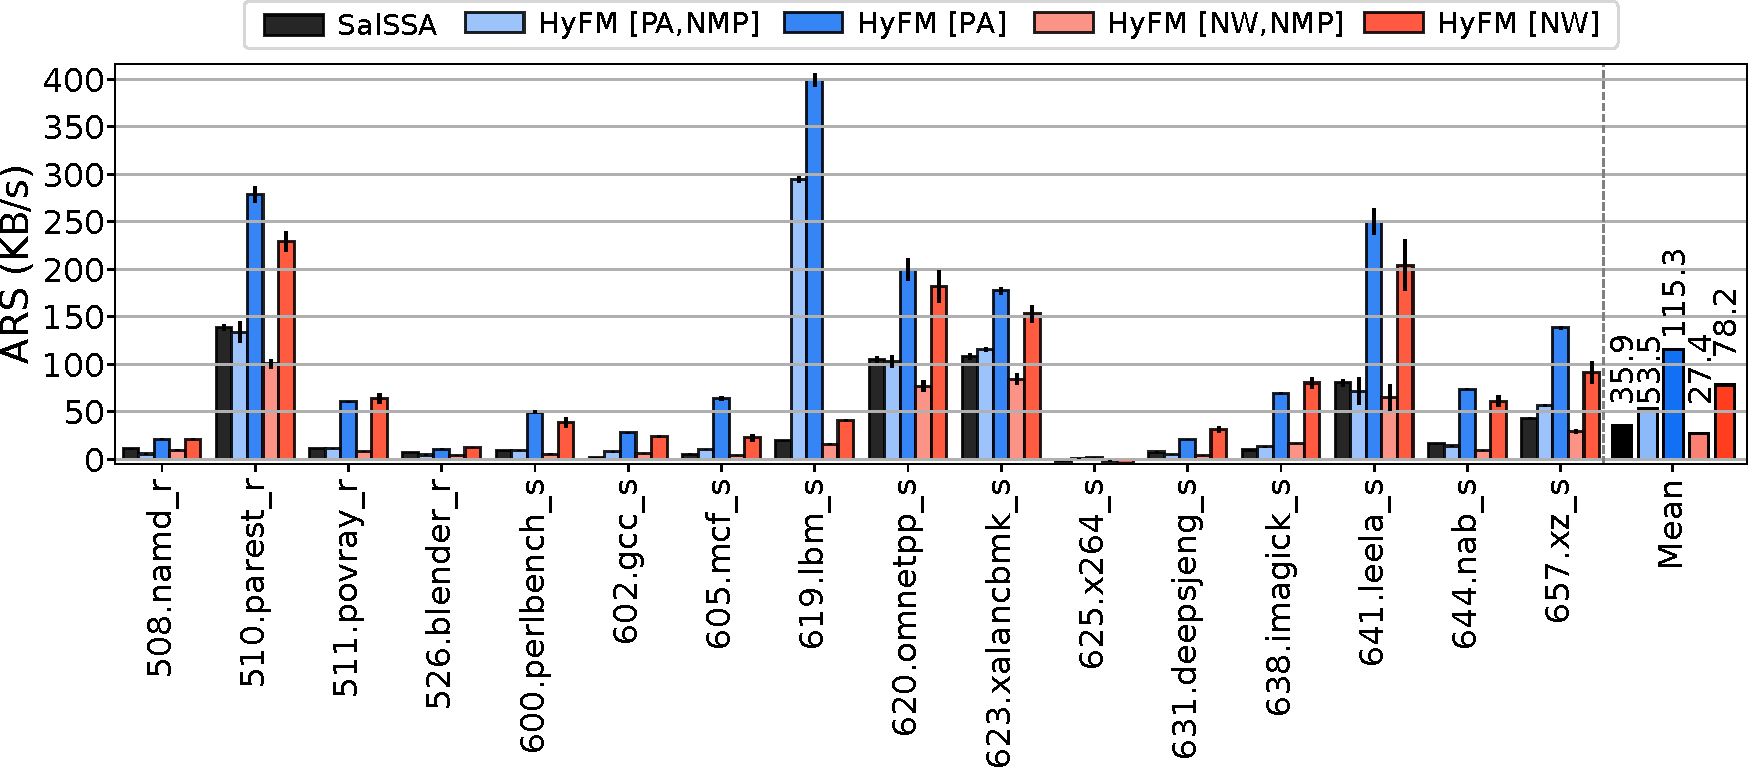
\includegraphics[width=\textwidth]{src/lctes21/figs/ars-spec17.pdf}
 \caption{SPEC CPU 2017.}
 \label{fig:ars-spec17}
 \end{subfigure}
 \caption{Average reduction speed on both SPEC 2006 and 2017.}
  \label{fig:ars-both}
 \end{figure}

%\begin{figure*}[h]
%  \centering
%  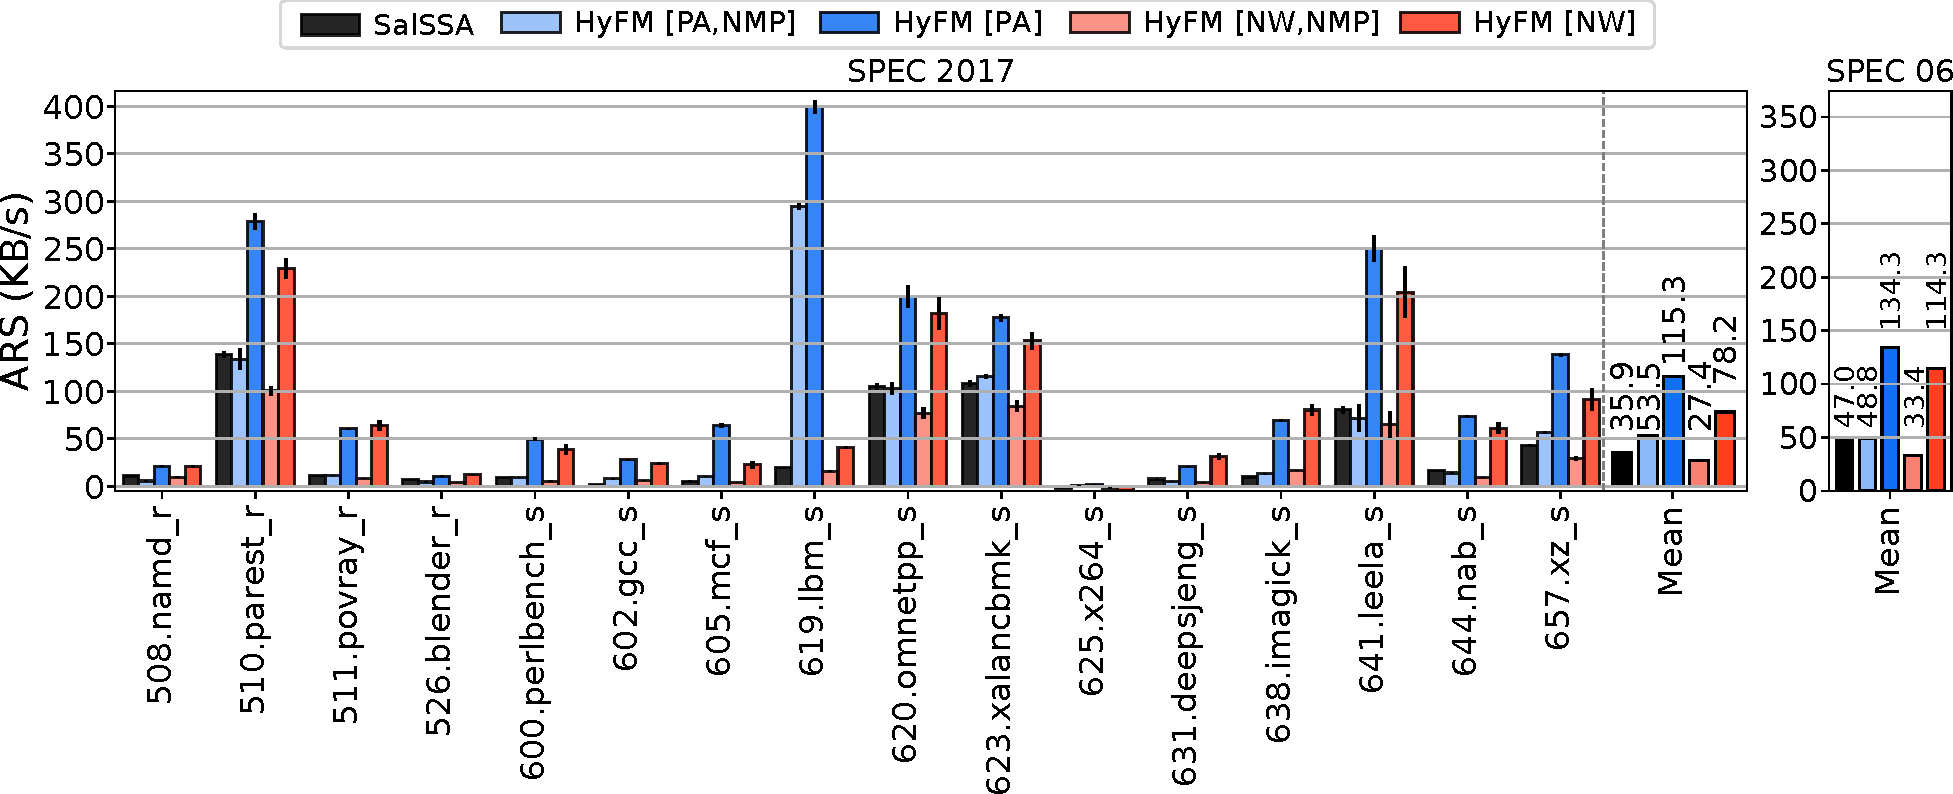
\includegraphics[width=0.95\linewidth]{src/lctes21/figs/ars-spec17-06.pdf}
%  \caption{Average reduction speed on both SPEC 2006 and 2017.}
%  \label{fig:ars-both}
%\end{figure*}

\subsection{Memory Usage} \label{sec:eval:memory}

 \begin{figure}[h]
   \centering
 \begin{subfigure}{\textwidth}
 \center
   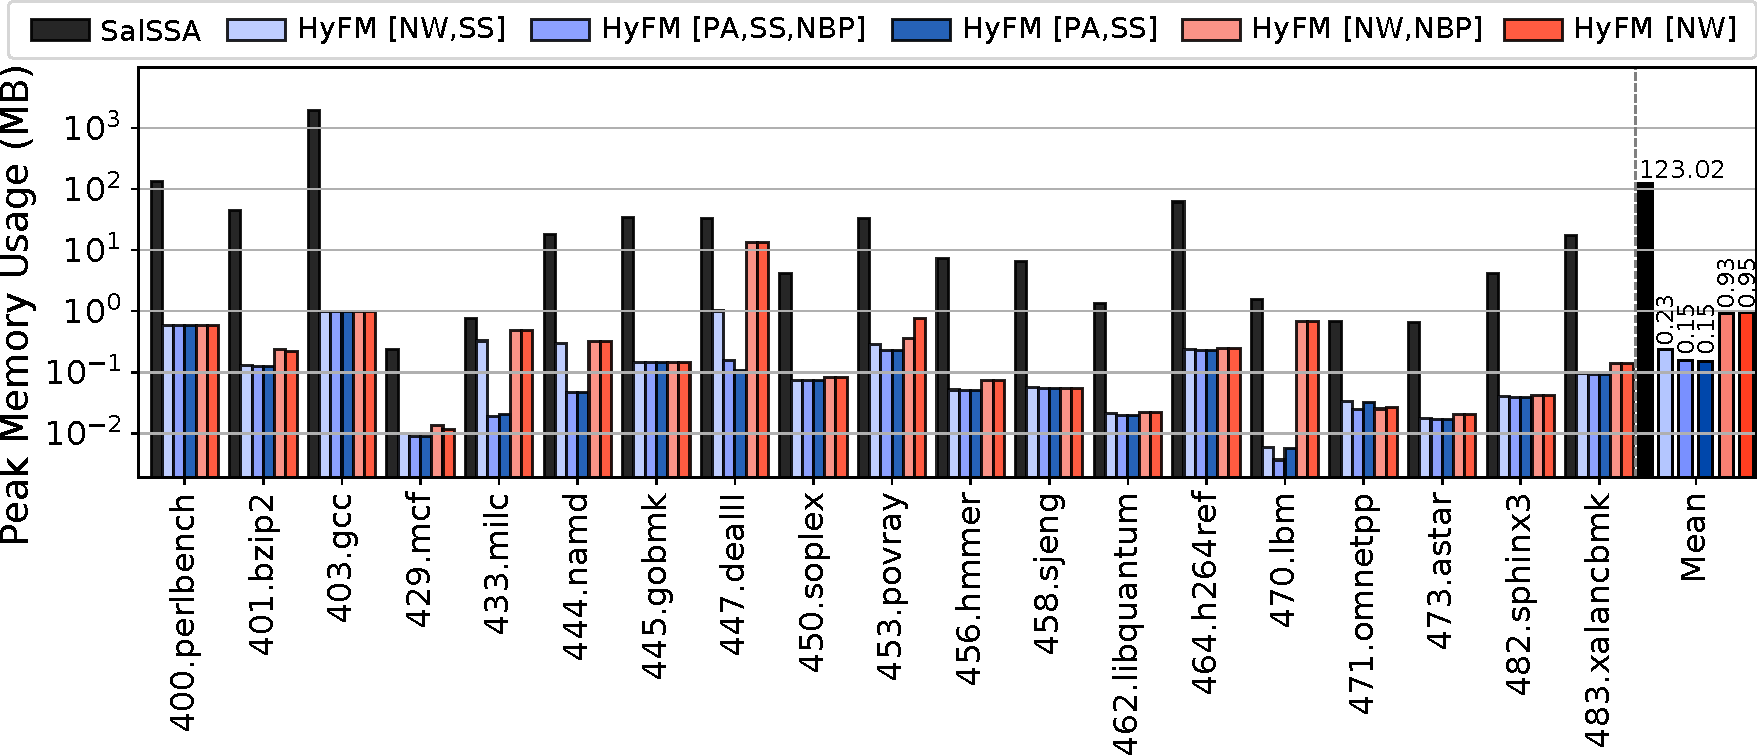
\includegraphics[width=\textwidth]{src/lctes21/figs/memory-spec06.pdf}
 \caption{SPEC CPU 2006.}
 \label{fig:memory-spec06}
 \end{subfigure}
 \\
 \begin{subfigure}{\textwidth}
 \center
   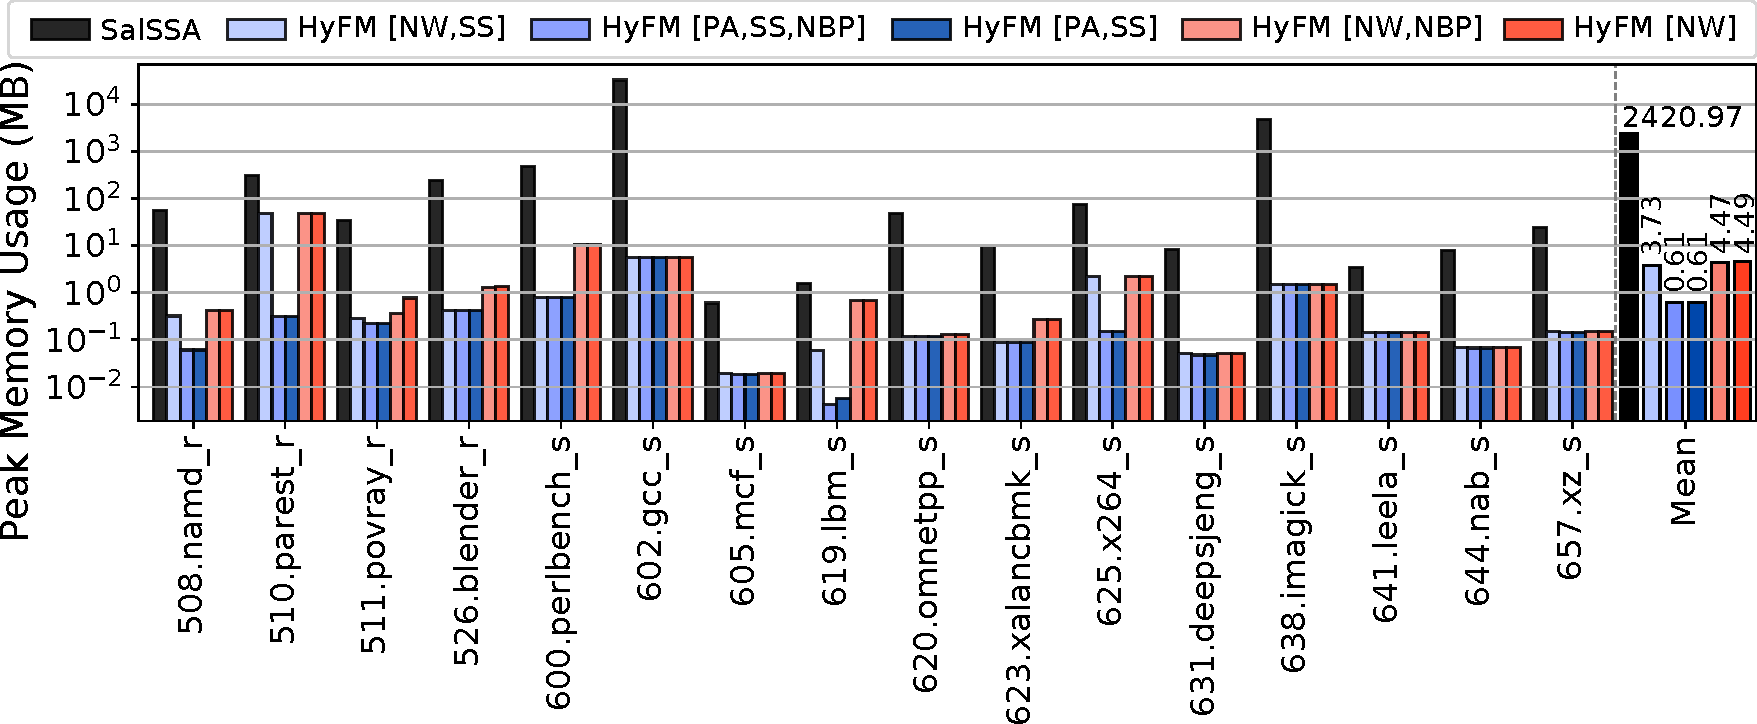
\includegraphics[width=\textwidth]{src/lctes21/figs/memory-spec17.pdf}
 \caption{SPEC CPU 2017.}
 \label{fig:memory-spec17}
 \end{subfigure}
 \caption{Peak memory usage of {\SOAName} and {\ProjName} variants for SPEC 2006 and 2017 in log scale. {\SOAName} has a peak memory usage several orders of magnitude hundreds higher than all other approaches. The pairwise alignment variants of {\ProjName} need on average only a seventh of the memory needed by the {\NW} variants.}
  \label{fig:memory-both}
 \end{figure}

%\begin{figure}[h]
%  \centering
%  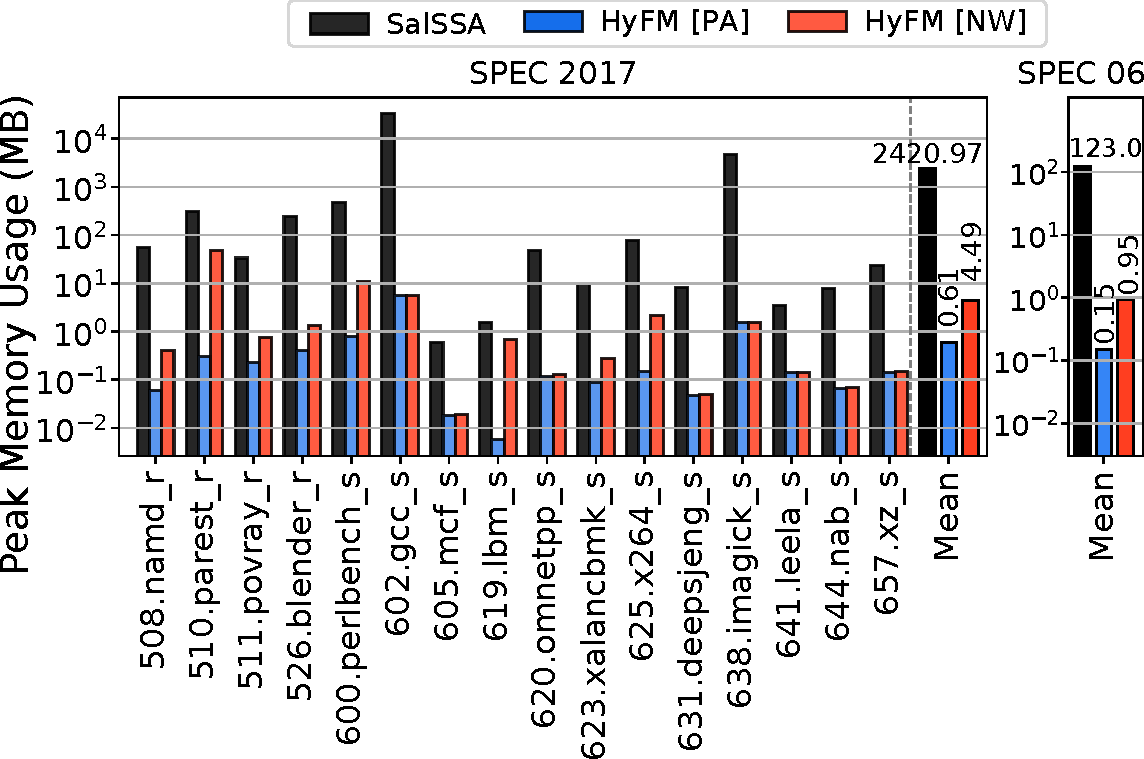
\includegraphics[width=\linewidth]{src/lctes21/figs/memory-spec17-06-tiny.pdf}
%  \caption{Peak memory usage of {\SOAName} and {\ProjName} variants for SPEC 2006 and 2017 in log scale. {\SOAName} has a peak memory usage several orders of magnitude hundreds higher than all other approaches. The pairwise alignment variants of {\ProjName} need on average only a seventh of the memory needed by the {\NW} variants.}
%  \label{fig:memory-both}
%\end{figure}

Another important aspect of function merging is peak memory usage. This is especially critical for an optimization designed for LTO.
Compilation in full LTO mode is already memory hungry. Just keeping the whole program in memory can be a significant problem for large programs~\cite{johnson17}. Maintaining additional information for every function and basic block could easily tip the compiler over the edge.

Figure~\ref{fig:memory-both} shows the peak memory usage (in log scale) needed for the alignment stage alone.
For {\SOAName}, this represents simply the execution of the {\NW} algorithm.
For {\ProjName}, the alignment stage represents both aligning each pair of basic blocks as well as the pairing these basic blocks.
Our results show that {[PA]} is over three orders of magnitude better than {\SOAName}, while {[NW]} is more than two orders of magnitude better.
In other words, while {\SOAName} requires on average 2.4~GB of memory, {[PA]} uses only around 610~KB and {[NW]} uses 5.6~MB.

The peak memory usage is especially noticeable on \texttt{gcc}, when merging its two largest functions, containing 90093 and 76265 instructions.
Since {\SOAName} applies its quadratic sequence alignment algorithm on the linearized sequences of the whole input functions, it uses over 32~GB of memory when merging these two functions.
Meanwhile, {[NW]} requires only around 5.6~MB for merging the same pair of input functions, even though it employs the same sequence alignment algorithm. This is because its peak memory usage is a quadratic function of the largest pair of \emph{blocks} instead of the largest pair of \emph{functions}.
Although very large, these two functions are composed of several thousands of very small basic blocks, so the memory overhead of {\NW} is limited.
Most of the memory consumed by {[NW]} in this case is actually needed for storing the basic block fingerprints.
This aspect becomes evident when we compare the peak memory usage of {[NW]} with that of the {[PA]} for \texttt{gcc}. They have similarly low memory requirements, even though only one of them uses a quadratic alignment algorithm.

In other cases, where basic blocks are longer, pairwise alignment leads to a significantly lower peak memory usage compared to {\NW}. For \texttt{parest}, for example, pairwise alignment reduces memory usage from \fixme{40}~MB to \fixme{200}~KB. Overall, {[PA]} needs around $6\times$ less memory. For smaller programs, {[NW]} might be a viable option but for larger ones being able to reduce memory usage to a minimum might be more important.

% \subsection{Summary}
% Overall, our novel function merging technique has surpassed the state-of-the-art in terms of compilation time, memory usage, as well as code size reduction.
% However, different variants of the proposed technique are better suited for different goals.
% If the code size is the utmost concern, {\ProjName}~[NW] is the winning strategy, but if we are looking for the most balanced trade-off between compilation-time overheads and code-size reduction, {\ProjName}~[PA] has shown better results.


\chapter{Conclusion} \label{chp:conclusion}

This thesis presents a novel compiler optimisation for reducing code size by merging functions.
Chapter~\ref{chp:fm-operation} describes our novel approach, based on sequence alignment, for merging any two functions.
Chapter~\ref{chp:opt-strategy} describes how our function merging technique can be combined with a optimisation strategy in order to search for profitable functions to merge, which includes a profitability cost model and a ranking of candidate functions.

This chapter is structured as follows:
Section~\ref{sec:conclusion:contribution} summarises the main contributions of this thesis,
%Section 7.2 presents a critical analysis of this work,
Section~\ref{sec:conclusion:futurework} describes future research directions,
and finally Section~\ref{sec:conclusion:summary}  provides concluding remarks.


% We have presented {\ProjName}, a novel compiler-based function merging technique with full support for the SSA form.
% Unlike the previous state-of-the-art, which has to apply register demotion to eliminate the commonly used \textit{phi-nodes} in SSA,
% {\ProjName} directly processes \textit{phi-nodes} using a more powerful code generator.
% As a result, {\ProjName} avoids the code bloating problem introduced by register demotion and
% increases the chances of generating profitable merged functions. We have implemented {\ProjName} in LLVM and evaluated it on the SPEC CPU2006
% and CPU2017 benchmark suites. {\ProjName} delivers on average 9.5\% code reduction for the lowest exploration threshold. Compared to the previous
% function merging state-of-the-art, {\ProjName} achieves $2\times$ more reduction on binary size with 3$\times$ less compile-time overhead and less than half the amount of memory required by it.

% We proposed a novel function merging approach based on sequence alignment, called FMSA. This was the first technique capable of merging any two functions, if deemed profitable, achieving up to 30\% of code-size reduction on SPEC 2006, about twice as much as the past state of the art.
% Although this technique offers significant improvements over previous ones, there are still many limitations and missed opportunities that prevent us from achieving all the available code compression.
% We need to improve the code generator, exploit code reordering, work at different scopes, scale to huge programs, avoid runtime slowdowns, work on JITs, and adopt machine learned heuristics.
% %To address these missed opportunities,
% %We plan to create a better code generator, a new approach that handles code reordering and merges code across different scopes, more accurate cost models
% %, with a better ranking mechanism and code aligner powered by deep learning.
% This will result in smaller programs without runtime or compile time overheads.

\section{Contribution} \label{sec:conclusion:contribution}

This thesis presents a novel function merging technique alongside an optimisation strategy.
Our novel technique uses sequence alignment algorithms from bioinformatics in order to identify the similarity between functions being merged.
The proposed optimisation is very effective at reducing code size by merging arbitrary functions.
Our approach does not suffer from any of the major limitations of existing solutions, outperforming them by more than 2.4$\times$.
We also proposed a ranking-based exploration mechanism to focus the optimization on promising pairs of functions.
Ranking reduces the compilation-time overhead by orders of magnitude compared to an exhaustive quadratic exploration. 
With this framework, our optimization is able to reduce code size by up to 25\%, with an overall average of about 6\%, while introducing an average compilation-time overhead of only 15\%.
Coupled with profiling information, our optimization introduces no statistically significant impact on performance.

\section{Future Work} \label{sec:conclusion:futurework}

For future work, we plan to focus on improving the ranking mechanism to reduce compilation time.
In order to avoid code size degradation, we also plan to improve the compiler's built-in static cost model for code size estimation.
We also plan to work on the linearisation of the candidate functions, allowing instruction reordering to maximize the number of matches between the functions.
Finally, we also plan to incorporate instruction reordering into function merging to maximize the number of matches between the functions regardless of the original code layout.
One can also investigate the application of phi-node coalescing outside function merging.
We envisage further improvements can be achieved by integrating the function-merging optimization to a summary-based  link-time optimization framework, such as ThinLTO in LLVM.
As a future work, we can also analyze the interaction between function merging and other optimizations such as inlining, outlining, and code splitting.

\subsection{Better Code Generator}

%FMSA's code generator is responsible for producing the actual merged functions from the aligned sequences.
%In its original version, FMSA has many artificial limitations in order to simplify its code generator.
%Preliminary results show that the code generator can be significantly improved, enabling far more code compression while reducing compilation time overhead.
%For this project, we plan to develop a new code generator that is capable of appropriately handling $\phi$-nodes, variable length arguments, calling convention, and exploiting target specific instructions to better compress code.
%There are still many opportunities to optimize operand selection and branch instructions that result from merging code. 

In order to better compress code, one can improve the code generator, optimising the parameters used as function identifiers based on calling conventions, exploit target specific instructions, and optimize operand selection and branch instructions that result from merging code.
There are also many missing features in the code generator that are important for its application in the industry.
For example, a new code generator could also be able to appropriately handle variable length arguments, and debug information.
When merging functions, having an optimised code generator is as important as optimally identifying which instructions to merge.
%In the industry, it is also crucial that we appropriately handle debug information when generating code. %link with: \phi$-nodes, variable length arguments
%Appropriately generating code with debug information is crucial for its application in the industry.

\subsection{Handling Code Reordering}

All existing function merging techniques rely on the order in which instructions appear inside the basic blocks and their arrangement,
failing to profitably merge equivalent functions when confronted even with the smallest variations on the ordering of instructions and basic blocks.
Figure~\ref{fig:code-reordering} shows an example of two functions that all existing techniques fail to merge even though they are obviously identical.
Our current technique produces the merged function shown in Figure~\ref{fig:merged-code-reordering}, which is considered unprofitable as it is unable to reduce code size.
Note that all indexing computation is duplicated, including the increment operation, resulting in a merged function that is unnecessarily bigger than the two original functions together.
We need more powerful graph, rather than sequence, alignment techniques to better identify and merge differently ordered but semantically equivalent code.

\begin{figure}[h]
 \centering
 \begin{subfigure}{.5\textwidth}
         \centering
         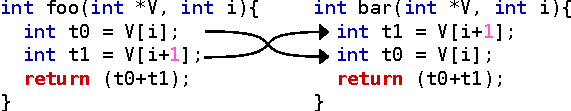
\includegraphics[scale=0.85]{src/conclusion/figs/motivation-1-code.pdf}
         \vspace{1ex}
         \caption{Two equivalent functions.}
         \label{fig:code-reordering}
 \end{subfigure}\begin{subfigure}{.5\textwidth}
         \centering
         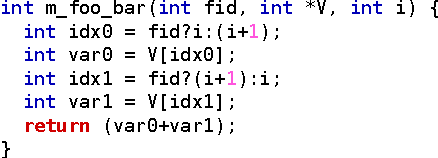
\includegraphics[scale=0.85]{src/conclusion/figs/motivation-1-merged-code.pdf}
         \caption{Merged function currently produced by FMSA.}
         \label{fig:merged-code-reordering}
 \end{subfigure}
    \vspace{-2ex}
    \caption{Example of how even trivial reordering is poorly handled by the existing solutions.}
    \label{fig:code-reordering-example}
\end{figure}

\subsection{Merging Across All Scopes}

Existing techniques are limited to one particular scope.
While function merging is applied only to whole functions,
function outlining is commonly applied at the basic block level.
%In one end we have an optimization such as the function outlining which is capable of merging or extracting equivalent basic blocks, in the other end we have function merging capable of merging whole functions.
However, equivalent code can be found within or across functions, which themselves may reside in the same source file or be spread across multiple source files.
Therefore, we need to develop a novel unified optimization capable of merging semantically equivalent code that can span anything between a single basic block up to a whole function.
This unification has the extra benefit of also addressing the phase ordering problem by coordinating the merge operations on different scopes.

\subsection{Scaling for Large Programs}

Although our optimisation achieves very good results in terms of code compression, it is still unable to handle large programs in a real scenario.
Its time complexity and memory usage requirements would prevent it from optimizing large programs such as web browsers, Clang/LLVM, and operating systems, as these programs tend to have many functions with several thousands of instructions.
Link-time optimization (LTO) makes this matter even worse by optimizing the code after the whole program has been linked into a single module, imposing a huge pressure on memory usage and compilation time.

%In this project, we will investigate this scalability issue.
%We plan to perform link-time optimization in an incremental fashion, such as using ThinLTO, which operates on individual translation units, reducing memory usage while also making it suitable for parallel and distributed compilation.
The optimization of different translation units can be distributed across different machines and merge operations locally performed in parallel.
In order for this to work, an important challenge that needs to be addressed concerns ranking and merging functions that reside in different translation units.
However, this is essential to enable the use of LTO on real programs while keeping the memory usage and compilation time acceptable.

\subsection{Powered by Deep Learning}

In order to reduce compilation time while also being effective, 
the ranking-based exploration mechanism tries to efficiently focus the search 
only to the most promising pairs of functions.
However, the existing solution is still very wasteful as most of the merged functions are
discarded by the profitability analysis.
Identifying what would be profitably merged is a very challenging task.

Given our group's expertise on the area, we plan to use solutions based on deep learning to efficiently predict which pairs of functions are most likely to be profitable to merge.
This approach has the potential to reduce compilation time even further while also improving the compression by finding profitable candidates that are currently missed.
Having accurate target-specific cost models is crucial for the effectiveness of the profitability analysis.
We plan to explore the use of machine learning techniques to develop more accurate cost models.

One can investigate the use of deep learning to align two functions and better identifying what can be merged.
Sequence alignment focusses only on maximizing the number of merged instructions,
without necessarily minimizing the number of operand selections or branches.
A smarter approach that understands how instructions interact with each other would be
very beneficial.


\subsection{Avoiding Performance Overheads}

For many real applications, it is desirable to achieve a good balance between code size and performance.
Preliminary results show that performance degradation can be completely avoided by using profiling to
guide the merging decisions.
One can avoid adding branches inside hot execution paths, therefore avoiding performance penalties.
Although hot code can be merged, it is important to minimize unnecessary branches when merging hot code.
We will develop a profile-guided optimization that automatically identify the best trade-off between code-size and performance.

\subsection{Less Memory Usage by JIT}

Ahead-of-time and just-in-time (JIT) compilation have completely different requirements.
Function merging can be used to reduce the amount of memory used by programs running on a JIT environment.
However, our solution must be adapted to the requirements that are specific to a JIT environment, as JIT compilers have the extra challenge of having to optimize the code as fast as possible.
This would require the development of completely new algorithms for ranking and aligning functions that are suitable for this application domain.
Another possibility is to exploit the fact multiple programs may be simultaneously running on the same JIT environment and merge code across different programs, reducing the overall memory usage.

\section{Summary} \label{sec:conclusion:summary}

